\sloppy
\chapter{Meta-Task: A Method-Agnostic Framework for Learning to Regularize in Few-Shot Learning}
\label{chap:meta_task}

\begin{figure}
  \centering
   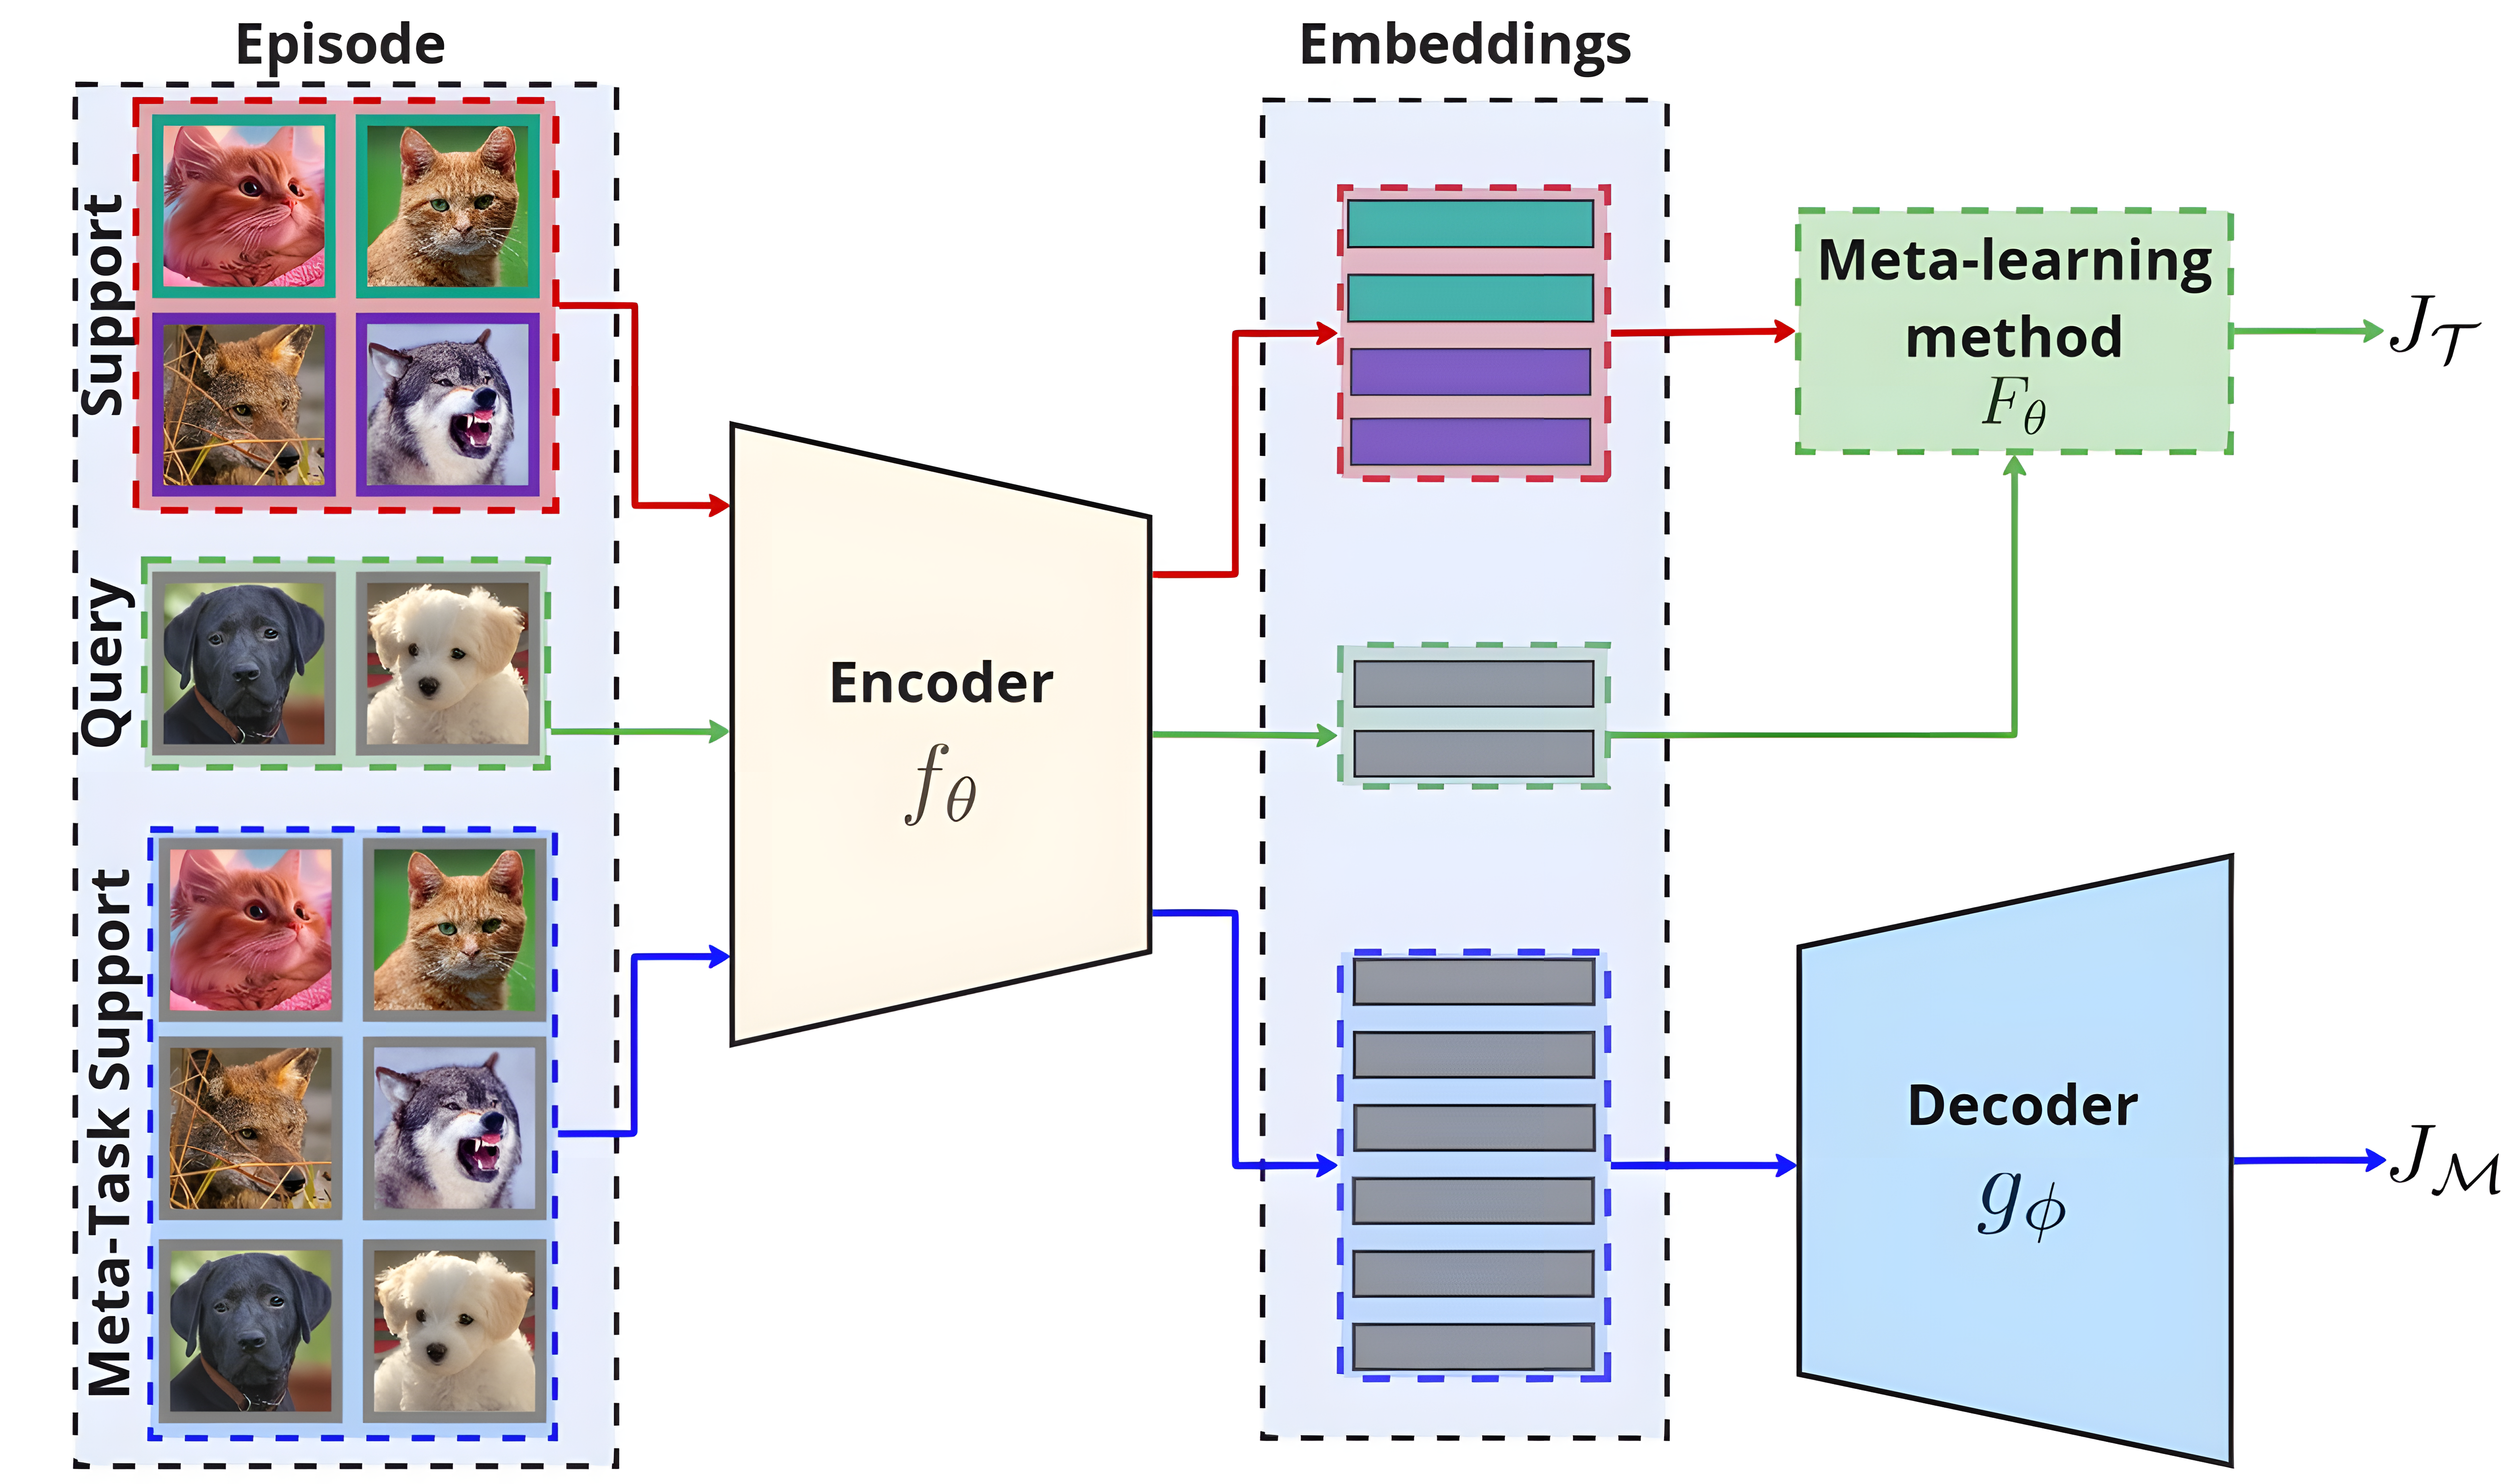
\includegraphics[width=1\linewidth]{FIGURES/metatask/meta-tasks.png}
   \caption{Detailed architecture of the Task-Decoder within the Meta-Task framework. The Meta-Task support set consists of unlabeled copies of support and query samples, which are fed into an encoder \( f_{\theta} \) to produce feature embeddings. These embeddings serve two key functions: (1) they are passed to a decoder \( g_{\phi} \) to reconstruct the input images, aiding in the learning of rich, meaningful representations, and (2) they are used to generate the meta-learning method ($F_{\theta}$) for query image classification. The model optimizes two objectives: classification loss (\( J_{\mathcal{T}} \)) and reconstruction loss (\( J_{\mathcal{M}} \)), each with a dedicated backpropagation step. The overall training loss is \( J_{\mathcal{T}} + \lambda J_{\mathcal{M}} \), balancing both classification accuracy and representation learning. For a broader application, the decoder \( g_{\phi} \) could be replaced by one or more neural networks that solve various unsupervised tasks.}

   \label{fig:1}
\end{figure}

\section{Introduction}
\label{sec:intro}

% Few-Shot Learning (FSL) has emerged as a promising solution to the problem of limited data availability in computer vision tasks. By employing meta-learning techniques, FSL approaches enable models to learn how to learn \cite{learn2learn} from a small number of instances, allowing effective generalization to novel tasks with minimal training data. The primary goal of FSL is to efficiently extract {\color{meaningful, transferable representations from sparse datasets.}} Recent advancements in deep learning, particularly in meta-learning, have led to powerful FSL techniques such as Matching Networks \cite{matching}, Relation Networks \cite{relation}, Model-Agnostic Meta-Learning (MAML) \cite{maml}, Prototypical Networks \cite{proto}, and Reptile \cite{reptile}.

% FSL enables models to recognize anomalies and uncommon occurrences, which is instrumental in medical applications and personalized health and nutritional recommendation systems \cite{nayem2023few, PFM_Ali, Event_Ali}. By reducing the data required to train a model, FSL can significantly lower the costs associated with data collection and annotation \cite{metasgd, support, metagan}.

% Despite significant progress in meta-learning \cite{learn2learn}, FSL models often suffer from overfitting, limiting their ability to generalize effectively to unseen tasks. Regularization is crucial for preventing overfitting and ensuring good generalization. In meta-learning, regularization involves both \textit{adaptation-generalization} and \textit{meta-generalization}% (see Glossary)
% . While conventional regularization methods from other areas of machine learning—such as weight decay \cite{krogh1991simple}, dropout \cite{hinton2012improving}, and noise injection \cite{achille2018information, alemi2016deep, tishby2015deep}—are applicable to meta-learning, specialized techniques have proven more efficient \cite{imaml, mrmaml, pan2021meta, wang2023improving, yao2021meta, yao2021improving, rajendran2020meta}.

% Motivated by these challenges, we propose a novel, method-agnostic framework called Meta-Task. This framework introduces auxiliary tasks designed specifically to regularize individual tasks during meta-learning. (%see Glossary and 
% Figure \ref{fig:1}). By treating regularization as a learnable task, we introduce an additional loss function that is optimized alongside the main tasks. This approach helps simplify the process of selecting suitable regularization terms that meet the needs of all tasks. It also allows for the integration of unsupervised or semi-supervised tasks as mechanisms for regularization.

\IEEEPARstart{F}\noindent ew-Shot Learning (FSL) has emerged as a promising solution to the problem of data scarcity in machine learning, particularly in computer vision, medical applications, and personalized health systems\cite{nayem2023few, PFM_Ali, Event_Ali}. By leveraging meta-learning, FSL enables models to learn how to learn\cite{learn2learn} with the primary objective of extracting meaningful, transferable representations from sparse datasets, reducing the need for extensive labeled data, and significantly lowering data collection and annotation costs~\cite{metasgd, support, metagan}. In wireless communications, where foundation models must rapidly adapt to diverse modulation schemes and channel conditions, FSL offers a practical solution. Rather than exhaustive retraining for each deployment scenario, meta-learning enables adaptation with minimal labeled data, a critical capability for cost-effective foundation model deployment.

Advances in meta-learning have led to techniques such as Matching Networks~\cite{matching}, Relation Networks~\cite{relation}, Model-Agnostic Meta-Learning (MAML)\cite{maml}, Prototypical Networks\cite{proto}, and Reptile~\cite{reptile}. Despite performance gains, FSL models remain prone to overfitting, limiting generalization.

Regularization plays a critical role in mitigating overfitting and enhancing generalization in FSL. Conventional methods such as weight decay\cite{krogh1991simple}, dropout\cite{hinton2012improving}, and noise injection\cite{achille2018information, alemi2016deep, tishby2015deep} fail to address FSL-specific challenges. Meta-learning requires both adaptation-generalization and meta-generalization\cite{imaml, mrmaml, pan2021meta, wang2023improving, yao2021meta, yao2021improving, rajendran2020meta}, yet existing techniques remain static, inflexible, and reliant on manually designed loss functions or auxiliary tasks that do not adapt to the unique structure of each task. This limitation motivates the need for a more dynamic, learnable regularization mechanism.

To address this limitation, we introduce Meta-Task, a method-agnostic framework that reformulates regularization as a learnable task within the FSL optimization process. Meta-Task dynamically learns task-specific regularization strategies through a parameterized neural layer $\phi$. This adaptive mechanism enables our framework to seamlessly integrate with existing FSL pipelines, ensuring flexibility across different task distributions and learning paradigms. Meta-Task remains compatible with existing auxiliary tasks and regularization losses, leveraging prior techniques while introducing a dynamic, learnable component. This enhances overfitting mitigation without extensive hyperparameter tuning or task-specific modifications, making it scalable and practical for real-world FSL applications.

To operationalize Meta-Task regularization, we propose using an autoencoder-based Task-Decoder (Figure \ref{fig:1}). The Task-Decoder serves as a flexible and effective regularizer, refining task-specific representations by constraining the embedding vector to reconstruct the original input accurately. We choose autoencoders because they are data-agnostic, easy to implement, architecturally flexible, and allow tunable parameterization for optimization. This adaptability makes them well-suited for various FSL applications, as they can seamlessly integrate into different model architectures.

Our method leverages the latent variable $z$, inherently present in most FSL settings due to the N-Way, K-Shot paradigm. The standard inner-outer loop optimization structure ensures the existence of an intermediate latent representation within the support-query split or gradient-based adaptation process. This guarantees compatibility across various FSL architectures, allowing Meta-Task to enhance regularization effectiveness dynamically.

The main contributions of this paper are as follows. (1) Meta-Task Framework: We propose Meta-Task, a novel, method-agnostic framework that introduces auxiliary tasks to regularize individual tasks in FSL. (2) Task-Decoder (Figure \ref{fig:1}): We introduce the Task-Decoder, utilizing autoencoders as a new regularization task for meta-learners, leveraging unsupervised learning to refine hidden representations. (3) Improved Performance: Our method demonstrates faster convergence, higher accuracy, and better generalization than existing techniques, all without extensive hyperparameter tuning. (4) Versatility and Applicability: The framework is method-agnostic and can be integrated with various FSL settings, making it suitable for real-world, resource-constrained scenarios.

\textbf{Framework Position:} Within the dissertation's modular framework, Meta-Task provides the rapid adaptation mechanism essential for wireless foundation models. While DenoMAE (Chapter~\ref{chap:denomae}) learns robust representations and the Plug-and-Play LLM (Chapter~\ref{chap:plugandplay}) enables training-free reasoning, Meta-Task addresses the critical challenge of adapting to new wireless scenarios with only 5-10 labeled examples. This few-shot capability is vital for cost-effective deployment across diverse channel conditions, modulation types, and operational environments. These are scenarios where acquiring extensive labeled data is prohibitively expensive. Meta-Task's method-agnostic design ensures compatibility with various architectures, making it a practical adaptation layer for wireless foundation models.

The remainder of the paper is organized as follows: Section \ref{sec:back_ground} reviews related work to contextualize the problem. Section \ref{sec:approach} details our proposed approach, and Section \ref{sec:results} presents experimental results. Finally, conclusions are drawn in Section \ref{sec:meta_tasks_conclusion}.


% \begin{table}[!ht]
% \caption*{\large\textbf{Glossary}}
% \resizebox*{0.5\textwidth}{!}{\begin{tabular}{l|p{5cm}}
% \textbf{Term}             & \textbf{Definition}            \\
% \hline
% method-agnostic            & Applicable to different meta-learning methods. \\
% FSL                       & Few-Shot Learning. \\
% support set               & Labeled examples for training. \\
% query set                 & Examples used for evaluation during training and testing.\\
% base task                 & A task used during the training phase of the model.\\
% novel task                & Unseen task for evaluation.  \\
% adaptation-generalization & Generalizing to specific tasks. \\
% meta-generalization       & Generalizing to new tasks. \\
% Meta-Task                 & Auxiliary task with parameter $\phi$ for regularization. \\
% regularization            & Preventing overfitting during training. \\
% Task-Decoder              & Component that decodes the appropriate weight regularization during training. \\

% \end{tabular}}
% \caption{Important terminology for understanding Meta-Task Framework}
% \label{glass}

% \end{table}


% \begin{figure*}[!ht]
%   \centering
%    \includegraphics[width=\linewidth]{images/proto.jpg}
%    \caption{A High-level view of Meta-Learning: Each episode is made up of labeled examples (the support set) and unlabeled instances (the query set). After that, the episode is fed into an embedding model, which maps the samples to a feature space, resulting in a compact representation of the episode. The meta-learning approach then uses this feature representation to learn and extract relevant information from the support set. Using the learned patterns and relationships from the support set, the obtained knowledge is applied to predict or make inferences on the query set.}
%    \label{fig:2}
% \end{figure*}

%------------------------------------------------------------------------

\section{Related Work}\label{sec:back_ground}

Here we position Meta-Task within this landscape.

Existing regularization approaches include Explicit Regularization (ER), Episode Augmentation Regularization (EAR), Task Augmentation Regularization (TAR), and Adversarial Task Upsampling (ATU)~\cite{imaml,mrmaml,yamaguchi2023regularizing,yao2021meta,wu2022adversarial}. While effective, these methods often require extensive pre-training, synthetic data generation, or task-specific modifications.

Meta-Task distinguishes itself by introducing a learnable, task-specific regularization strategy through a parameterized neural layer $\phi$ that dynamically adapts without modifying the underlying FSL architecture. Unlike iMAML~\cite{imaml} and MR-MAML~\cite{mrmaml} (which focus on meta-initialization and gradient regularization) or ProtoDiff~\cite{du2023protodiff} (which requires computationally intensive diffusion models), Meta-Task learns robust embeddings during meta-training through auxiliary tasks, making it method-agnostic, computationally efficient, and suitable for resource-constrained environments.


\begin{table}[ht]
\centering
\caption{Comparison of meta-learning regularization methods.}
\resizebox*{0.7\textwidth}{!}{
\begin{tabular}{lccccc}
\toprule
\textbf{Method} & \textbf{Category} & \textbf{Method-Agnostic} & \textbf{Complexity} \\
\midrule
{iMAML} \cite{imaml} & ER & No & Medium
\\
{MR-MAML} \cite{mrmaml} & ER & No & Medium \\ 
{Minimax-Meta} \cite{wang2023improving} & ER & No & Low \\
{DAC-MR} \cite{shu2023dac} & EAR & Yes & Medium \\
{MetaMix} \cite{chen2021metamix} & EAR & Yes & Medium \\
% \textbf{Channel Shuffle} \cite{yao2021improving} & TAR & Yes & Low \\
{ProtoDiff} \cite{du2023protodiff} & TAR & No & High \\
{ATU} \cite{wu2022adversarial} & TAR & Yes & High \\
{LEO} \cite{leo} & ER & No & High \\
\textbf{Task-Decoder (Ours)} & \textbf{MTR} & \textbf{Yes} & \textbf{Medium} \\
\bottomrule\\
\end{tabular}
}
\caption*{The table compares various meta-learning regularization techniques by category, method-agnostic capability, and computational complexity. Categories include Explicit Regularization (ER), Episode Augmentation Regularization (EAR), Task Augmentation Regularization (TAR), and our proposed Meta-Task Regularization (MTR).}
\label{tab:meta_learning_comparison}

\end{table}

% \subsection{Prototypical Networks}

% Prototypical Networks~\cite{proto} are a class of few-shot learning models that represent each class by the mean of its support examples (the prototype) in an embedding space. Classification of query samples is performed based on the distance to these prototypes, typically using Euclidean distance. The embedding function $f_{\theta}$ is learned to project input images into a feature space where samples of the same class are close together.

% \subsection{Model-Agnostic Meta-Learning (MAML)}

% MAML~\cite{maml} is a meta-learning algorithm that aims to find initial model parameters that can be quickly adapted to new tasks with a few gradient updates. It does so by optimizing for parameters with maximal sensitivity to changes in the task, facilitating rapid learning on new tasks.


% \begin{figure}[!ht]
%   \centering
%    \includegraphics[width=0.5\linewidth]{images/prototypical.jpg}

%    \caption{The embedding space that prototypical network create for embedding $\{Z_{n_k}\}_{k=1}^{K}$}
%    \label{fig:z}
% \end{figure}
%------------------------------------------------------------------------

\section{Meta-Task Framework}\label{sec:approach}

While our framework is domain-agnostic and demonstrated on image classification benchmarks, it is particularly motivated by wireless foundation models where rapid adaptation to new scenarios (channel conditions, modulation types) with minimal labeled data is essential for economical deployment. The method operates on learned representations regardless of whether they originate from images, wireless signals represented as images (spectrograms, constellation diagrams), or other modalities.

In this section, we introduce our proposed Meta-Task Framework, a novel approach that enhances generalization by integrating learnable Meta-Tasks as a form of regularization. By treating regularization itself as a learnable task, our framework encourages the model to develop richer and more robust feature representations. The framework is method-agnostic and can be seamlessly integrated with existing FSL models, such as Prototypical Networks and MAML. In the following subsections, we detail the components of the framework, including the Task-Decoder, the problem formulation, and the theoretical justification for its effectiveness.

Our framework extends MAML \cite{maml} by introducing regularization as a \textit{learnable Meta-Task}, enabling unsupervised task integration during meta-training without requiring additional data. The following subsections detail the implementation and theoretical foundations of our contributions:

\begin{itemize}
\item \textbf{Task-Decoder:} We introduce an unsupervised autoencoder architecture that implements our learnable regularization concept by reconstructing input images from their embeddings, proving its effectiveness in enriching feature representations.
\item \textbf{Problem Formulation:} We present the mathematical framework that enables the integration of unsupervised auxiliary tasks with existing FSL methods, demonstrating how our approach remains method-agnostic through separable loss functions.
\item \textbf{Theoretical Analysis:} We provide theoretical justification for our framework's convergence properties and establish how the joint optimization of primary and Meta-Tasks enhances generalization capabilities.
\end{itemize}

\subsection{Task-Decoder}

At the core of our Meta-Task Framework is the Task-Decoder (Figure \ref{fig:1}), an unsupervised learning component designed to enhance the embedding space by reconstructing input images from their embeddings. The Task-Decoder employs an autoencoder architecture, where the encoder \( f_{\theta} \) maps the input images to a latent embedding space, and the decoder \( g_{\phi} \) reconstructs the images from these embeddings.

By encouraging the embeddings to retain sufficient information for accurate reconstruction, the Task-Decoder prevents the encoder from focusing solely on discriminative features that may not generalize well. This leads to richer and more robust feature representations, ultimately improving the model's performance on unseen tasks.

The Task-Decoder operates in parallel with the primary few-shot learning model, processing the same inputs and contributing to the overall learning objective through its reconstruction loss.

\subsection{Problem Formulation}

Let the Meta-Task $\mathcal{M}$ denote the Task-Decoder, and our meta-learning method $F$ be Prototypical Networks. We define the encoder network \( f_{\theta} \) parameterized by \( \theta \), and \( g_{\phi} \) represent the decoder network parameterized by \( \phi \). 

For a given query sample \( x\in\mathcal{Q} \) and its true class \( y \) belonging to task $\mathcal{T}$, the Prototypical Network $F_{\theta}$ computes class prototypes using support set $\mathcal{S}$ and classifies $x$ based on the closest prototype to the embedding $f_{\theta}$.

\noindent
\textbf{Primary Task Loss:} The probability of \( x \) belonging to class \( n \) is:

\begin{equation} p_{\theta}(y={n} \mid x) = \frac{\exp\left(-d\left(f_{\theta}(x), c_{{n}}\right)\right)}{\sum_{k=1}^{N} \exp\left(-d\left(f_{\theta}(x), c_k\right)\right)}, \end{equation}
where $N$ is the number of tasks in the episode, \( c_n \) is the prototype of class \( n \) and \( d(\cdot, \cdot) \) denotes the Euclidean distance. The classification loss is then:

\begin{equation}
J_{\mathcal{T}}(x, \theta) = -\log p_{\theta}(y = n \mid x).
\end{equation}

\noindent
\textbf{Meta-Task Loss:} The Task-Decoder aims to reconstruct \( x \) from \( f_{\theta} \), with the reconstruction loss defined as:

\begin{equation}
J_{\mathcal{M}}(x, \theta, \phi) = \left\| g_{\phi}(f_{\theta}(x)) - x \right\|^2.
\end{equation}

\noindent
\textbf{Combined Loss Function:} The total loss for a sample \( x \) is a weighted sum of the primary task loss and the Meta-Task loss:

\begin{equation}
J(x, \theta) = J_{\mathcal{T}}(x, \theta) + \lambda J_{\mathcal{M}}(x, \theta, \phi),
\end{equation}
where \( \lambda \) is a hyperparameter balancing the two losses or the learning rate for the Meta-Task update.

\noindent
\textbf{Optimization:} The model parameters \( \theta \) and \( \phi \) are optimized jointly over all tasks and samples. For a given task $\mathcal{T}$, the overall loss is calculated by summing the combined losses over all query samples:

\begin{equation}\label{eq:task_loss}
J_{\mathcal{T}}(\theta) = \sum_{x \in \mathcal{T}} J_{\mathcal{T}}(x, \theta). 
\end{equation}

During meta-training, we sample a batch of tasks $\{\mathcal{T}_i\}^L_{i=1}$. The total loss across all tasks in an episode is:

\begin{equation}\label{eq:overall_loss_separate}
J(\theta) = \sum_{i=1}^{L} \left(J_{\mathcal{T}_i}(\theta) + \lambda J_{{\mathcal{M}_i}}(\theta, \phi)\right).
\end{equation}

By minimizing this combined loss, the model learns embeddings that are both discriminative for classification and informative for reconstruction, enhancing generalization across tasks. The full algorithm of the Task-Decoder integration is provided in Algorithm~\ref{alg:task_decoder}.

We define tasks and Meta-Tasks as separable if their loss functions can be computed independently and summed without including interaction terms. This structure allows us to optimize each component separately while still contributing to the overall objective. If the regularization term is separable (as in our case with the autoencoder), we can simplify \eqref{eq:overall_loss_separate} as
\begin{equation}\label{eq:9}
J(\theta) = \sum_{i=1}^{L} J_{\mathcal{T}_i}(\theta) +\lambda\sum_{i=1}^{L}J_{{\mathcal{M}_i}}(\theta,\phi).
\end{equation}

If each task may have multiple or no Meta-Tasks attached, the overall loss function generalizes to:
\begin{equation}\label{eq:10}
J(\theta) = \sum_{i=1}^{L} J_{\mathcal{T}_i}(\theta) +\lambda\sum_{r=1}^{R}J_{{\mathcal{M}_r}}(\theta,\phi),
\end{equation}
where $R$ is the total number of regularizers applied to the model.

\subsection{Justification}

Our Meta-Task framework provides unique theoretical guarantees, distinguishing it from existing regularization approaches. In Equations \eqref{eq:9} and \eqref{eq:10}, we demonstrated that incorporating auxiliary tasks into training effectively reformulates the FSL paradigm to a new FSL setting with a combined distribution of primary tasks and Meta-Tasks, denoted as 
$\mathcal{T}'$. This reformulation allows the overall training objective to be expressed as a sum over $L+R$ tasks, preserving the structure necessary for standard FSL optimization techniques.

When using MAML as the FSL method, based on convergence guarantees proven in literature~\cite{wang2022global}, our approach converges to an optimal set of parameters for $\mathcal{T}'$. Since the Meta-Tasks are carefully designed to enhance generalization, this optimal parameter set enables the model to generalize effectively across both primary tasks and Meta-Tasks. The convergence of $\phi$ to its global optima further ensures that the learned embeddings retain the essential information necessary for both classification and reconstruction. This joint optimization ($\theta$) constructs a globally optimal representation space, improving overall model performance on unseen tasks by reducing generalization error.

A critical advantage of Meta-Task is the separability of the primary and auxiliary tasks. Since their loss functions can be computed independently, optimization can proceed efficiently, with each task contributing to the overall objective. This design simplifies the optimization process and supports convergence to a global optimum, as the auxiliary tasks act as an implicit regularizer, reducing overfitting by penalizing non-generalizable embeddings.

A rigorous mathematical proof is more challenging for FSL methods beyond MAML. However, as all FSL methods aim to optimize parameters that generalize across task distributions with limited examples, it is reasonable to infer that our approach improves generalization capabilities, as demonstrated in the results section. Additional experiments, including visualizations of reconstructed features in Section~\ref{sec:feature_analysis}, empirically validate how Meta-Task enhances embedding quality and task generalization.

\begin{remark}{The proposed regularization approach is method-agnostic and can be applied to any FSL learning method.} \end{remark}
\begin{remark}{Equations \eqref{eq:9}, \eqref{eq:10} hold only if tasks and Meta-Tasks are separable or independent.}
\end{remark}
\begin{remark}{The use of autoencoders is because autoencoders can be used with any type of data, are easy to use, and are flexible in architecture.}
\end{remark}

\begin{algorithm}[t]
\caption{Meta-Tasks: Task-Decoder}
\label{alg:task_decoder}
\begin{algorithmic}[1]
\REQUIRE $p(\mathcal{T})$: distribution over tasks; 
\REQUIRE $f_{\theta}$: embedding network;
\REQUIRE $g_{\phi}$: decoder network; 
\REQUIRE $\alpha$, $\lambda$: learning rates;
\REQUIRE $F$: meta-learning method (e.g., Prototypical Networks);
\REQUIRE $J_{\mathcal{T}}(x, \theta)$: classification loss;
\\$J_{\mathcal{M}}(x, \theta, \phi) = \| g_{\phi}(f_{\theta}(x)) - x \|^2$: reconstruction loss

\STATE Randomly initialize $\theta$ and $\phi$
\WHILE{not done}
    \STATE Sample support set: $\mathcal{S} \sim p(\mathcal{T})$
    \STATE Sample query set: $\mathcal{Q} \sim p(\mathcal{T})$
    \STATE Compute reconstruction loss:\\
    $~~~~~~~~~~~~~~~~~{J}_{\mathcal{M}}(\theta, \phi) \leftarrow \frac{1}{|\mathcal{S} \cup \mathcal{Q}|} \sum_{x \in \mathcal{S} \cup \mathcal{Q}} J_{\mathcal{M}}(x, \theta, \phi)$
    \STATE Use the support set $\mathcal{S}$ and embedding network $f_{\theta}$ to get meta-learning method $F_{\theta}$.
    \STATE Compute classification loss on query set:\\
    $
    ~~~~~~~~~~~~~~~~~~~~{J}_{\mathcal{T}}(\theta) \leftarrow \frac{1}{|\mathcal{Q}|} \sum_{x \in \mathcal{Q}} J_{\mathcal{T}}(x, F_{\theta})
    $
    \STATE Update embedding network parameters:\\
    $
    ~~~~~~~~~~~~~~~~~~~~\theta \leftarrow \theta - \alpha \nabla_{\theta} \left( {J}_{\mathcal{T}}(\theta) + \lambda {J}_{\mathcal{M}}(\theta, \phi)) \right)
    $
    \STATE Update decoder parameters:\\
    $
    ~~~~~~~~~~~~~~~~~~~~~~~~~~\phi \leftarrow \phi - \lambda \nabla_{\phi} {J}_{\mathcal{M}}(\theta, \phi)
    $
\ENDWHILE
\end{algorithmic}
\end{algorithm}


\section{Experiments and Results}\label{sec:results}

We validate Meta-Task on standard computer vision benchmarks to demonstrate its general applicability and enable comparison with existing FSL methods. This validation establishes the framework's effectiveness on vision few-shot tasks; Section~\ref{sec:wireless_meta_task} then tests directly whether the same mechanism transfers to a wireless AMC deployment.

In this section, we conduct comprehensive experiments to validate the effectiveness of our proposed {Meta-Task} framework in enhancing generalization and mitigating overfitting in few-shot learning. Our objectives are to: 
\begin{enumerate} 
\item Demonstrate that incorporating Meta-Tasks as auxiliary regularization improves model generalization to both seen and unseen tasks.
\item Validate that leveraging both labeled and unlabeled data through an unsupervised autoencoder refines hidden representations.
\item Showcase the method-agnostic applicability of {Meta-Task} across various FSL settings and its practical efficiency in resource-constrained scenarios. 
\end{enumerate}

We begin by outlining the experimental setup, including datasets, model architectures, and implementation specifics. Following this, we present our results along with a comprehensive analysis of our findings, focusing on the impact of the {Meta-Task} framework on performance, convergence speed, and variance reduction.

\subsection{Datasets}

We evaluated the proposed {Meta-Task} framework on three standard benchmarks commonly used in few-shot learning:

\noindent
\textbf{MiniImageNet}~\cite{mini-imagenet}: This dataset consists of 100 classes selected from ImageNet, with 600 images per class resized to $84 \times 84$ pixels. It is divided into 64 training, 16 validation, and 20 test classes, ensuring that test classes are entirely disjoint from training classes for robust evaluation of generalization capabilities.

\noindent
\textbf{TieredImageNet}~\cite{ren2018meta}: A larger and more challenging dataset comprising 608 classes organized into 34 high-level categories, providing semantic diversity. It includes 351 training, 97 validation, and 160 test classes, with images resized to $84 \times 84$ pixels. Its hierarchical structure makes it suitable for evaluating models' ability to generalize across different levels of abstraction.

\noindent
\textbf{FC100}~\cite{oreshkin2018tadam2}: Derived from the CIFAR-100 dataset, FC100 contains 100 classes, each with 600 images resized to $32 \times 32$ pixels. The dataset is split into 60 training, 20 validation, and 20 test classes. It presents unique challenges due to low-resolution images and high intra-class variability, making it an excellent benchmark for assessing model robustness.

These datasets offer diverse and challenging scenarios for few-shot learning, enabling us to thoroughly evaluate the generalization capabilities of the {Meta-Task} framework.

\subsection{Methods}

To demonstrate the method-agnostic nature of our approach, we integrated the {Meta-Task} framework with four few-shot learning models:

\noindent
\textbf{Prototypical Network (PN)} \cite{proto}: Utilizes a ResNet-18 \cite{resnet} backbone for feature extraction. It computes class prototypes in the embedding space, classifying query samples based on their distances to these prototypes.

\noindent
\textbf{MAML}~\cite{maml}: Employs a four-layer ConvNet architecture aiming to find initial model parameters that can be quickly adapted to new tasks with minimal gradient updates.

\noindent
\textbf{MetaOptNet}~\cite{lee2019meta}: Uses a ResNet-12 backbone and incorporates differentiable convex optimization layers for efficient classification, seamlessly integrating with our {Meta-Task} framework.

{\color{black} \noindent
\textbf{P$>$M$>$F} \cite{pmf}: Uses DINO\cite{dino} framework as its backbone. Like PN, it computes class prototypes in the embedding space. It classifies query samples based on their distances to these prototypes but with the added benefit of leveraging pre-trained transformer-based feature extraction.}

In our {Meta-Task} framework, we introduced a Task-Decoder employing an unsupervised autoencoder to reconstruct input images from their embeddings. The decoder mirrors the encoder architecture used in the backbone models. This process leverages both labeled and unlabeled data (support and query sets), refining the hidden representations and mitigating overfitting.

For the autoencoder architecture, we experimented with different configurations to assess the impact of the Task-Decoder's depth on performance. Specifically, we used both shallow and deep autoencoders, with parameters ranging from 75K to 250K. The shallow autoencoder consists of two convolutional layers, while the deep autoencoder includes four convolutional layers. This allowed us to analyze how the complexity of the Task-Decoder affects the overall performance.

We trained all models using the Adam optimizer with learning rates set to $1 \times 10^{-4}$ for the encoder and classifier, and $1 \times 10^{-6}$ for the Task-Decoder. Each model was trained over 50,000 episodes using 5-way 1-shot and 5-way 5-shot scenarios. The query size was maintained at 15 for both training and evaluation phases. To enhance model robustness, we applied standard data augmentation techniques, including random cropping, horizontal flipping, and color jittering.

Furthermore, we investigated the effect of using multiple autoencoders per task by associating different autoencoders with specific layers of the encoder network. However, we found that using a single autoencoder provided a good trade-off between performance improvement and computational overhead. %The complete source code and results for this paper can be found in the following GitHub repository: {HIDDEN}
 %\ref{https://github.com/woreom/meta-learning}{https://github.com/woreom/meta-learning}.

%%%%%%%%%%%%%%%%%%%%%%%%%%%%%%%%%%Loss%%%%%%%%%%%%%%%%%%%%%%%%%%%%%%%%%%
\begin{figure}[htbp]
  \centering
  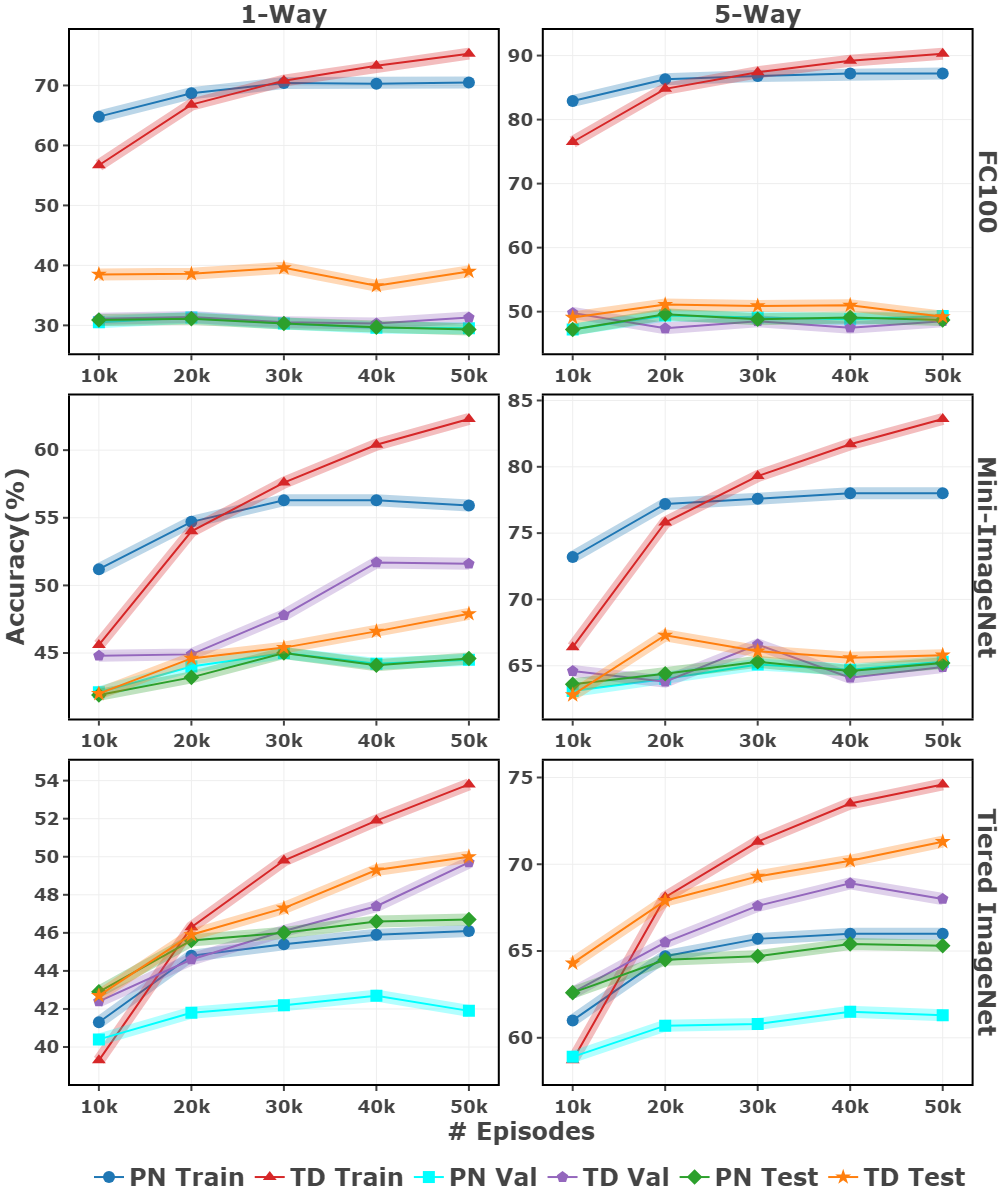
\includegraphics[width=1\linewidth]{FIGURES/metatask/acc_2.png}
  \caption{Accuracy curves for Prototypical Networks (PN) and Task-Decoder (TD) across different datasets, plotted against the number of episodes.}
  \label{fig:5}
\end{figure}

\begin{figure}[htbp]
  \centering
  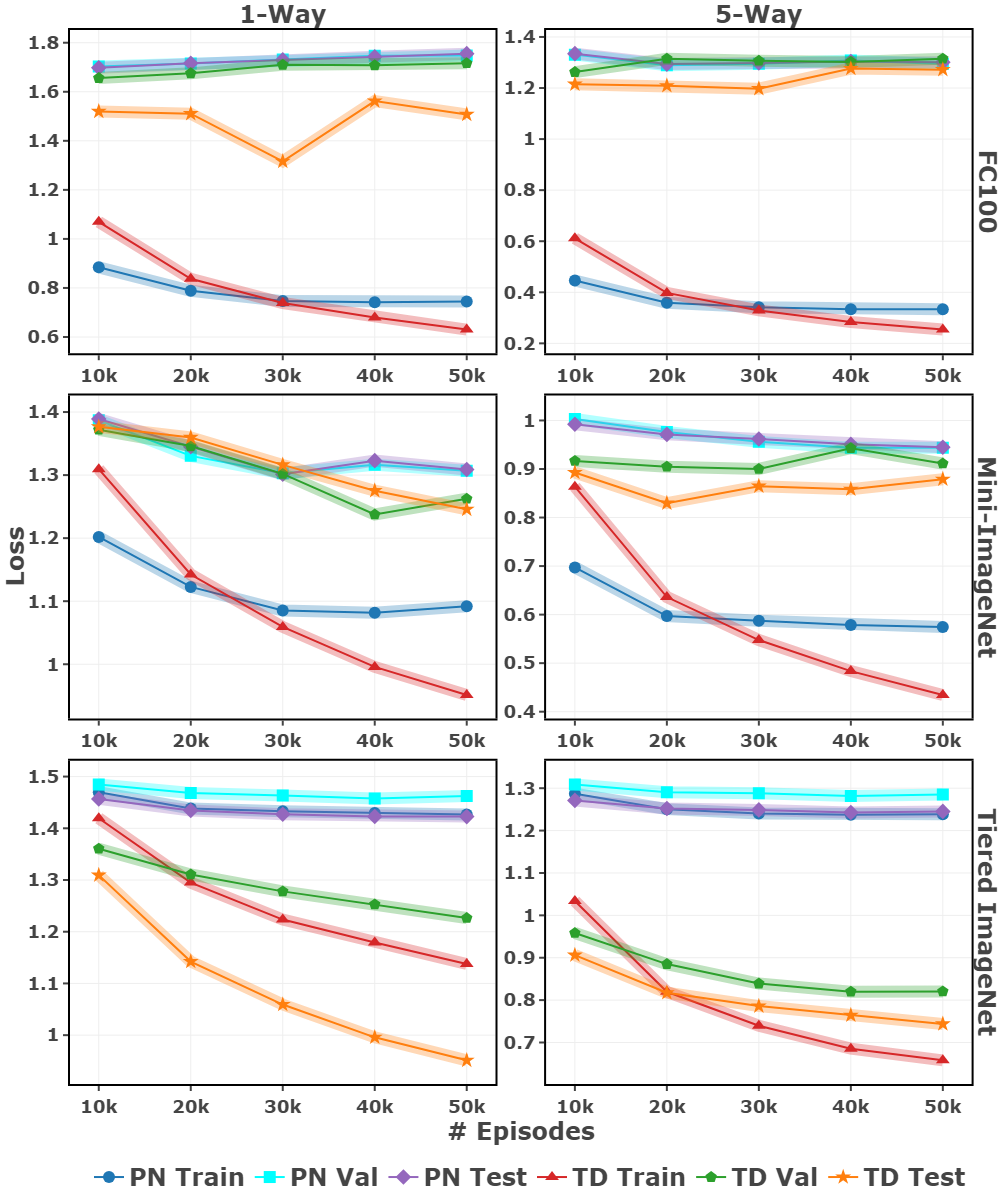
\includegraphics[width=1\linewidth]{FIGURES/metatask/loss_2.png}
  \caption{Loss curves for Prototypical Networks (PN) and Task-Decoder (TD) across different datasets, plotted against the number of episodes.}
  \label{fig:4}
\end{figure}
%%%%%%%%%%%%%%%%%%%%%%%%%%%%%%%%%%TABLE%%%%%%%%%%%%%%%%%%%%%%%%%%%%%%%%%%
\begin{table*}[htbp]
\centering
\caption{Comparison of few-shot classification accuracies (\%) with standard deviation on MiniImageNet and TieredImageNet datasets.}
\label{table:1}
\resizebox{\textwidth}{!}{%
\begin{tabular}{ll|cccc}
\toprule
                                               &                    & \multicolumn{2}{c}{MiniImageNet}                                        & \multicolumn{2}{c}{TieredImageNet}                                          \\
Method                                         & Backbone           & \multicolumn{1}{l}{5-way 1-shot(\%)} & \multicolumn{1}{l}{5-way 5-shot(\%)} & \multicolumn{1}{l}{5-way 1-shot(\%)} & \multicolumn{1}{l}{5-way 5-shot(\%)} \\
\hline & & \\
PN                           & ResNet18           & 45                          & 65.2                            & 46.6                            & 65.4                            \\
\textbf{PN(TD)}  & ResNet18           & \textbf{47.9 }              & \textbf{66.1 }                  & \textbf{50 }                    & \textbf{71.3 }                  \\
MAML                                           & CNN                & 47.54                        & 62.23                            & -                                    & -                                    \\
\textbf{MAML (TD)}                   & Shallow CNN Decoder                & \textbf{47.81}               & \textbf{62.52}                   & -                                    & -                                    \\
\textbf{MAML (TD)}                   & CNN & \textbf{47.67}               & \textbf{63.01}                   & -                                    & -                                    \\
Relation Networks\cite{relation}      & 64-96-128-256      & 50.44 ± 0.82                     & 65.32 ± 0.70                         & 54.48 ± 0.93                         & 71.32 ± 0.78                         \\
R2D2\cite{bertinetto2018meta}                   & 96-192-384-512     & 51.2 ± 0.6                       & 68.8 ± 0.1                           & -                                    & -                                    \\
Transductive Prop Nets\cite{liu2018learning} & 96-192-384-512     & 55.51 ± 0.86                     & 69.86 ± 0.65                         & 59.91 ± 0.94                         & 73.3 ± 0.75                          \\
SNAIL\cite{mishra2017simple}                   & ResNet-12          & 55.71 ± 0.99                     & 68.88 ± 0.92                         & -                                    & -                                    \\
AdaResNet\cite{munkhdalai2018rapid}              & ResNet-12          & 56.88 ± 0.62                     & 71.94 ± 0.57                         & -                                    & -                                    \\
TADAM \cite{oreshkin2018tadam2}                 & ResNet-12          & 58.5 ± 0.30                      & 76.7 ± 0.30                          & -                                    & -                                    \\
MetaOptNet                                     & ResNet-12          & 61.23 ± 0.29                     & 77.14 ± 0.21                         & 63.10 ± 0.34                         & 78.58 ± 0.27                         \\
\textbf{MetaOptNet (TD)}             & ResNet-12          & \textbf{61.35 ± 0.29}            & \textbf{77.3 ± 0.22}                 & \textbf{63.20 ± 0.34}                & \textbf{78.66 ± 0.27}\\
{\color{black}P$>$M$>$F}                                     & \color{black}IN1K,ViT-base          & \color{black}\textbf{72.80 }                     & \color{black}\textbf{90.70 }                         & -                         & -                        \\
{\color{black}\textbf{P$>$M$>$F(TD)}}             & \color{black}IN1K,ViT-base          & \color{black}\textbf{74.10 }            & \color{black}\textbf{92.30 }                 & -                & -\\
\bottomrule
\end{tabular}%
}
\caption*{\textit{Note:} Results are reported for 5-way 1-shot and 5-way 5-shot. `PN' and `TD' refer to Prototypical Networks and Task-Decoder, respectively.}
\end{table*}

\begin{table}[htbp]
\centering
\caption{Comparison of few-shot classification accuracies (\%) with standard deviation on the FC100 dataset \cite{oreshkin2018tadam2}.}
\label{table:2}
\resizebox{0.7\textwidth}{!}{%
\begin{tabular}{l|cc}
  \toprule
                                              &  \multicolumn{2}{c}{FC100}                                                   \\
Method                                         & \multicolumn{1}{l}{5-way 1-shot(\%)} & \multicolumn{1}{l}{5-way 5-shot(\%)} \\
\hline & & \\
PN                            & 31.1                            & 49.6                            \\
\textbf{PN (TD)}  & \textbf{39 }                    & \textbf{51.1 }                  \\
TADAM\cite{oreshkin2018tadam2}                  & 40.1 ± 0.4                           & 56.1 ± 0.4                           \\
MetaOptNet                                     & 40.19 ± 0.25                         & 55.04 ± 0.26                         \\
\textbf{MetaOptNet (TD)}             & \textbf{40.59 ± 0.26}                & \textbf{55.38 ± 0.25}                \\
\bottomrule
\end{tabular}%
}
\caption*{\textit{Note:} Results are reported for 5-way 1-shot and 5-way 5-shot settings. `PN' and `TD' refer to Prototypical Networks and Task-Decoder, respectively.}
\end{table}
%%%%%%%%%%%%%%%%%%%%%%%%%%%%%%%%%%TABLE%%%%%%%%%%%%%%%%%%%%%%%%%%%%%%%%%%
\subsection{Performance Evaluation}
{\color{black} 
Our experimental results demonstrate that the Meta-Task framework consistently outperforms baseline models across all datasets and settings, achieving higher accuracy with significantly fewer training episodes. For example, as shown in Figure~\ref{fig:5}, TD enables higher test accuracy within 20k episodes, whereas PN Test fails to achieve the same even after 50k episodes. Similarly, in Table~\ref{table:1}, TD P$>$M$>$F reaches 92.30\% accuracy in 3k episodes compared to P$>$M$>$F's 90.70\% after 4k episodes.

These results highlight the framework's efficiency in leveraging a small number of additional parameters to enhance generalization while reducing computational overhead. By introducing Meta-Tasks, the learning process is effectively regulated, eliminating the need for extensive parameter tuning or large-scale episodic training. This makes the Meta-Task framework both lightweight and practical for real-world applications. Further details on are provided in Table~\ref{table:1} and Table~\ref{table:2}.

From a wireless foundation model perspective, these results validate the feasibility of rapid adaptation with minimal labeled data. The 5.9 percentage point improvement on TieredImageNet 5-way 5-shot (Table~\ref{table:1}) demonstrates that foundation models need not require extensive labeled datasets for each deployment scenario. The 20k vs. 50k episode convergence reduction translates directly to training cost savings, which is critical for economical wireless AI deployment across diverse channel conditions and modulation types.
}

\subsubsection*{Prototypical Network Results}
Table~\ref{table:1} presents our experimental results on MiniImageNet and TieredImageNet, where our proposed method, the Task-Decoder, demonstrates significant performance improvements over the baseline Prototypical Networks. Specifically, on TieredImageNet in the 5-way 5-shot setting, our approach achieved an increase from 65.4\% to 71.3\% in test set accuracy, reflecting a substantial 5.9\% absolute improvement. This gain indicates superior meta-generalization capabilities of our method.

In the 5-way 1-shot scenario, the Task-Decoder improved accuracy from 46.6\% to 50\% on TieredImageNet, highlighting its efficacy in scenarios with extremely limited data. These consistent improvements across different datasets and settings demonstrate the robustness and effectiveness of our approach.
\subsubsection*{MAML Results}
Table~\ref{table:1} also showcases the performance of the {Task-Decoder} integrated with MAML. Our method outperforms the baseline MAML by up to 0.27\% in the 5-way 1-shot setting and up to 0.78\% in the 5-way 5-shot setting on MiniImageNet. Although the absolute improvements are modest, they demonstrate the effectiveness of the {Task-Decoder} in enhancing the adaptability of MAML.

To examine the impact of the {Task-Decoder's} architecture ($\phi$) on generalization, we trained MAML using two different{Task-Decoders}: a shallow decoder with 75K parameters and a deeper decoder with 250K parameters. Interestingly, the shallow decoder excelled in the 5-way 1-shot task, suggesting that deeper models are not always superior when data is scarce. In contrast, the deeper decoder performed better with more shots, highlighting the importance of model depth in specific contexts. This indicates that the Task-Decoder and its Meta-Task extensions can be effective even with a shallow network, which is beneficial in resource-constrained environments.

It's important to note that MAML requires the computation of second derivatives during optimization. However, to remain consistent with our claim of a method-agnostic framework, we chose to use a first-order approximation for the Task-Decoder's optimization. This decision avoids the computational overhead associated with second-order derivatives but may introduce approximation errors. Another limitation may stem from the inherent difficulties of optimizing the learning rate in MAML, which is complicated by the need for careful tuning due to its sensitivity to hyperparameters. While using the same learning rate as the Prototypical Networks simplifies comparisons, it likely constrained MAML's overall performance. These factors suggest that further optimization and fine-tuning could enhance the benefits of integrating the Task-Decoder with MAML.

\subsubsection*{MetaOptNet Results}
The results presented in Table~\ref{table:1} indicate that integrating the Task-Decoder with MetaOptNet \cite{lee2019meta} leads to modest but consistent performance improvements, with an average accuracy increase of 0.12\% in the 5-way 1-shot setting and 0.16\% in the 5-way 5-shot setting on MiniImageNet. While these gains are not as pronounced as those observed with other methods, they underscore the potential of the Task-Decoder to enhance performance even in well-optimized frameworks like MetaOptNet.

We attribute the smaller improvements to MetaOptNet's distinctive training setup, where variations in batch size and the number of shots significantly impact model performance. Due to hardware limitations, we reduced the batch size and the number of training shots, which may have constrained the performance gains. These findings suggest that further hyperparameter optimization, such as adjusting batch size or learning rate, could yield more substantial improvements.

{\color{black} \subsubsection*{P$>$M$>$F Results}
Due to the pre-trained nature of the encoder, we implemented a custom scheduler to align TD's optimization. Additionally, hardware constraints necessitated deviations from the original hyperparameters, such as reducing image sizes and query shots, which may have influenced the observed improvements. Despite these constraints, TD achieved a notable 1.45\% performance increase, demonstrating its flexibility and adaptability to transformer-based methods under constrained conditions.}

\subsection{Regularization Improvements}
Figure~\ref{fig:5} illustrates that our method achieves higher accuracy more quickly during all training, validation, and testing phases compared to the baseline, which demonstrates faster convergence. Additionally, Figure~\ref{fig:4} illustrates that the loss associated with our method decreases more rapidly and consistently remains lower throughout the training process across all training, validation, and test sets. The Task-Decoder achieves a mean loss of 1.23 with a variance of 0.001, whereas the baseline has a mean loss of 1.3 and a variance of 0.0002. This indicates more efficient learning and improved generalization.

To address concerns regarding implementation specifics, we provide detailed information about the hyperparameters, training times, and autoencoder architectures in Section~\ref{sec:exp_details}. We also conducted ablation studies to analyze the effect of different autoencoder architectures and the use of multiple autoencoders per task. The results indicate that while deeper autoencoders can provide marginal performance gains, the computational overhead increases significantly. Therefore, a single, appropriately sized autoencoder strikes a good balance between performance and efficiency.


\section{Wireless Validation: Meta-Task for AMC on RadioML}
\label{sec:wireless_meta_task}

The vision benchmarks above establish that Meta-Task's learnable regularization helps few-shot generalization when the base learner has a weak inductive bias. This section asks the question those benchmarks cannot answer directly: \textit{does the same auxiliary task help when the backbone is a wireless signal encoder, the deployment is cross-dataset, and classification runs through the DiSC-AMC pipeline of Chapter~\ref{chap:plugandplay}?}

\subsection{Experimental Design}

We evaluate on RadioML 2018.01a (24 classes, five SNR levels from $-20$ to $+20$ dB), using the full DiSC-AMC pipeline (DeepSeek-R1-Distill-Qwen-7B reasoning over discretized, retrieval-augmented exemplars; Section~\ref{sec:disc_amc}) as the fixed downstream endpoint, so that any effect of the auxiliary task is measured on the metric that matters for the dissertation's RQ2 contribution, not on an encoder's classification head in isolation. We compare three configurations that isolate the Task-Decoder's effect while holding the encoder backbone (DenoMAE2.0) and the reasoning pipeline fixed:
\begin{description}
    \item[(A) DenoMAE2.0 baseline] the encoder frozen, only a classification head trained, as published in Chapter~\ref{chap:plugandplay}'s DiSC-AMC Scenario III results.
% TODO(author-audit): (A) is labelled frozen but cites Scenario III (fine-tuned, Table 4.5); 21.5 = mean of Table 4.5 DenoMAE2.0 DiSC-AMC column; Table 4.6 (unadapted) mean = 9.17. Reconcile label/reference.
    \item[(B) DenoMAE2.0, fine-tuned] the encoder updated end-to-end on RadioML, with no auxiliary task.
    \item[(C) DenoMAE2.0 + Meta-Task] identical to (B), with the Task-Decoder's reconstruction loss added on a separate optimizer.
\end{description}
The main comparison is \textbf{C vs.\ B}: the two configurations share the same backbone and fine-tuning protocol, differing only in whether the auxiliary task is present.

Two protocol fixes were necessary for this comparison to be fair, both motivated by an earlier result that did not survive scrutiny. An initial run with a \emph{frozen} encoder (Meta-Task's auxiliary loss added only to the classification head) showed a +4.6 percentage point gain at $-20$ dB. This gain disappeared once the comparison was corrected: \textbf{Fix 1} trains both the Task-Decoder and the vanilla fine-tuning baseline with real, matched end-to-end fine-tuning of the encoder (matching the protocol used for DINOv2 elsewhere in Chapter~\ref{chap:plugandplay}), rather than leaving the encoder frozen only for the Task-Decoder arm; \textbf{Fix 2} places the auxiliary reconstruction loss on its own optimizer with a small learning rate ($10^{-6}$), as in the original Meta-Task implementation (Section~\ref{sec:approach}), rather than folding it into the main loss via a scalar weight $\lambda$, which had been inflating its apparent effect.

\subsection{Results}

\begin{table}[htbp]
\centering
\caption{Wireless validation: DiSC-AMC pipeline accuracy on RadioML 2018.01a (24 classes), averaged over five SNR levels ($-20$ to $+20$ dB).}
\label{tab:metatask_wireless}
\begin{tabular}{lc}
\toprule
Configuration & Mean Accuracy (\%) \\
\midrule
% TODO(author-audit): (A) is labelled frozen but cites Scenario III (fine-tuned, Table 4.5); 21.5 = mean of Table 4.5 DenoMAE2.0 DiSC-AMC column; Table 4.6 (unadapted) mean = 9.17. Reconcile label/reference.
(A) DenoMAE2.0, frozen encoder & 21.5 \\
(B) DenoMAE2.0, fine-tuned, no auxiliary task & 23.0 \\
(C) DenoMAE2.0, fine-tuned + Meta-Task & 22.2 \\
\bottomrule
\end{tabular}
\end{table}

Table~\ref{tab:metatask_wireless} reports the result under the corrected protocol: \textbf{(C) 22.2\% vs.\ (B) 23.0\%}: Meta-Task's auxiliary task gives \emph{no net gain} over plain fine-tuning on this cross-dataset wireless AMC task, and is marginally, not significantly, below it. The one effect that held up under both protocol fixes is the end-to-end fine-tuning itself: moving from a frozen encoder to a fine-tuned one (A$\to$B) improves mean accuracy by +1.5 points (21.5\%$\to$23.0\%), confirming that adapting the backbone to the target domain matters, even though adding Meta-Task's regularization on top of that adaptation does not help further. For reference, DiSC-AMC with a fine-tuned DINOv2 backbone (Chapter~\ref{chap:plugandplay}, Table~\ref{tab:disc_scenario3}) still reaches 76.25\% at $+20$ dB on the same benchmark, an order of magnitude above any DenoMAE2.0 configuration here, which underscores that representation quality, not the regularizer, is the binding constraint on this dataset.

\subsection{Discussion: A Bounded, Honest Null Result}

We report this as a \textbf{robust null result}: both plausible objections to the initial positive finding (an unfair frozen-encoder comparison and an improperly weighted auxiliary loss) were checked explicitly, and neither reversal flips the conclusion. This matters for two reasons. First, it demonstrates the value of adversarial self-checking of promising early results before they are reported as a contribution; the original +4.6-point frozen-encoder result would have overstated Meta-Task's wireless applicability had it not been re-examined under a fair protocol. Second, it sharpens the dissertation's account of \emph{why} Meta-Task helps where it helps: Section~\ref{sec:results} showed its largest gains on metric learners with a weak inductive bias (Prototypical Networks) applied to within-domain few-shot vision tasks; here, the task is instead cross-dataset transfer (SynthMod-10-trained representations evaluated on RadioML), where Section~\ref{sec:disc_discussion} already identified the self-supervised \emph{representation} itself, not the classifier's regularization, as the bottleneck. A learnable auxiliary task cannot compensate for an encoder whose embeddings do not retrieve informative neighbors on the target dataset. This connects directly back to RQ1 (Chapters~\ref{chap:denomae}--\ref{chap:cdrf}): on wireless cross-dataset transfer, representation quality dominates regularization.

\section{A Second Wireless Test: Few-Shot Channel Estimation}
\label{sec:channel_estimation}

The RadioML experiment above tests Meta-Task on one wireless task. An independent study, Roshan et al.~\cite{roshan2026channelestimation} (second-author work of this dissertation, with R.~Gh.~Roshan first), asks the broader question that RQ3 poses for a different wireless task: can a model that has learned to adapt specialize to an unseen channel from only a few labeled examples? It does not use Meta-Task. It uses standard MAML and MultiGrade-MAML (MG-MAML), so it is evidence about learning-to-learn on wireless data, not about the Task-Decoder, and it is used here only as corroboration.

\subsection{Setup}

The task is pilot-aided channel estimation in a single-antenna OFDM system: reconstruct the full time-frequency channel response from a noisy least-squares (LS) estimate interpolated from sparse pilots, scored by mean squared error (MSE, lower is better). Source and target channels are simulated: five Tapped Delay Line profiles (TDL-A to TDL-E, at 0, 5, and 10 dB SNR, giving 15 channel conditions) and nine urban-microcell (UMi) conditions from the CeBed framework. Splits are made at the channel level, so each evaluated channel is unseen in training (10 of 15 TDL conditions and 4 of 9 UMi conditions are used for training). For each unseen channel, 5 labeled frames are used for fine-tuning and the remaining 226 frames for evaluation. Four estimators are compared under the same budget: LS; linear MMSE (LMMSE), which uses second-order channel and noise statistics; ChannelNet, a convolutional estimator trained without meta-learning; and the two meta-learners, MAML and MG-MAML.

\subsection{Results}

Table~\ref{tab:channel_est} combines the paper's NLOS, LOS, and domain-shift results. The UMi column is a domain shift, since the learned models were trained mostly on TDL channels.

\begin{table}[htbp]
\centering
\caption{Few-shot (5-shot) channel estimation MSE; lower is better. TDL-A and TDL-C are rich-multipath NLOS channels, TDL-D and TDL-E are LOS-dominant, and UMi is a domain shift. Values are as reported by Roshan et al.~\cite{roshan2026channelestimation}.}
\label{tab:channel_est}
\small
\resizebox{\linewidth}{!}{%
\begin{tabular}{lcccccc}
\toprule
Method & TDL-A (0 dB) & TDL-A (5 dB) & TDL-C (5 dB) & TDL-D (5 dB) & TDL-E (10 dB) & UMi (5 dB) \\
\midrule
LS (input) & 1.7326 & 0.5483 & 0.5490 & 0.5508 & 0.1759 & 0.1844 \\
LMMSE & \textbf{0.0202} & \textbf{0.0065} & \textbf{0.0075} & \textbf{0.0073} & \textbf{0.0024} & \textbf{0.0022} \\
ChannelNet & 0.1571 & 0.0742 & 0.0744 & 0.0432 & 0.0229 & 0.0258 \\
MAML & 1.4831 & 1.5827 & 1.1330 & 0.1926 & 0.2282 & 0.0563 \\
MG-MAML & 0.4366 & 0.4736 & 0.4170 & 0.0793 & 0.0482 & 0.1164 \\
\bottomrule
\end{tabular}}
\end{table}

Four observations follow from the table. First, the classical LMMSE estimator has the lowest error in every condition, because it uses explicit second-order statistics that act as a structural prior. Second, the learned estimators are sensitive to noise and channel complexity: in the NLOS conditions MAML's error is as large as, or larger than, that of the LS input it starts from (for example 1.5827 against 0.5483 on TDL-A at 5 dB), consistent with inner-loop gradients being estimated from five noisy frames. Third, the non-meta ChannelNet is better than both meta-learners in every condition shown, and MG-MAML, which stages the meta-updates for stability, is steadier than MAML on NLOS channels but is not robust to the UMi shift (0.1164, worse than ChannelNet's 0.0258). Fourth, increasing the number of adaptation frames helps the meta-learners but does not close the gap (Table~\ref{tab:channel_est_k}): MAML and MG-MAML improve from 1 to 10 shots, with a non-monotonic step for MAML at 15, while ChannelNet is nearly flat, and none approaches LMMSE's 0.0022.

\begin{table}[htbp]
\centering
\caption{Effect of the number of adaptation frames $K$ on UMi channel estimation (MSE; lower is better), from Roshan et al.~\cite{roshan2026channelestimation}.}
\label{tab:channel_est_k}
\begin{tabular}{lcccc}
\toprule
Model & 1-shot & 5-shot & 10-shot & 15-shot \\
\midrule
ChannelNet & 0.0291 & 0.0258 & 0.0263 & 0.0251 \\
MAML & 0.0902 & 0.0563 & 0.0508 & 0.0581 \\
MG-MAML & 0.1487 & 0.1164 & 0.0921 & 0.0870 \\
\bottomrule
\end{tabular}
\end{table}

\subsection{What It Adds to RQ3}

This study supports the RQ3 answer in three ways. It shows that the RadioML null result is not specific to Meta-Task, to classification, or to the DiSC-AMC pipeline: on a second wireless task, learning-to-learn did not reliably beat a plain learned estimator, and under noise and domain shift it was often worse. It suggests a mechanism that fits the RadioML finding, namely that adaptation from a handful of noisy examples amplifies variance, so what limits adaptation is the quality and generality of the starting representation or prior, not the adaptation procedure. And it supplies a counterpart to the dissertation's arc from hand-crafted features to learned representations (Section~\ref{sec:familiar_arc}): the estimator built on explicit channel statistics is the most robust under data paucity and shift, while learned priors are distribution-dependent.

The bounds are as important as the support. MAML and MG-MAML are not Meta-Task, and the task is regression on simulated channels rather than modulation classification, so the study does not test the Task-Decoder or the RadioML claim directly. The results are single reported values per condition without confidence intervals, and LMMSE benefits from channel statistics that the learned models must acquire from data. Whether Meta-Task's reconstruction objective, which is close in spirit to channel estimation viewed as image reconstruction, helps here is untested and is left to future work.

\section{Conclusion}\label{sec:meta_tasks_conclusion}


In this paper, we introduced Meta-Task, a method-agnostic framework that treats regularization as a learnable task for few-shot learning. By integrating an autoencoder-based Task-Decoder directly within the meta-learning optimization, our approach provides continuous, unsupervised regularization that prevents overfitting and improves generalization. Extensive experiments across multiple datasets (Mini-ImageNet, Tiered-ImageNet, FC100) and meta-learning methods (Prototypical Networks, MAML, MetaOptNet, P$>$M$>$F) demonstrate consistent improvements in accuracy, convergence speed, and cross-domain generalization.

\textbf{Connection to the Dissertation Framework:} Meta-Task provides a \emph{partial} answer to Research Question 3 (RQ3): \textit{Can a learnable auxiliary task improve generalization when only a few labeled examples exist?} On vision few-shot benchmarks, the answer is yes: Prototypical Networks improve from 65.4\% to 71.3\% on Tiered-ImageNet 5-way 5-shot, reaching the baseline's best accuracy in under 20k episodes versus more than 50k without the Task-Decoder, with consistent (if uneven) gains across MAML, MetaOptNet, and P$>$M$>$F. On the wireless deployment tested directly in Section~\ref{sec:wireless_meta_task}, however, Meta-Task gives no net gain over plain fine-tuning on cross-dataset RadioML AMC through the DiSC-AMC pipeline (22.2\% vs.\ 23.0\%). The lesson this bounded result supports is that \emph{on wireless cross-dataset transfer, the representation is the bottleneck, not the regularizer}: Meta-Task's adaptation layer is most valuable when the base learner's inductive bias is weak and the domain is in-distribution, and is not a substitute for a better encoder (Chapters~\ref{chap:denomae}--\ref{chap:cdrf}) when the encoder itself fails to transfer. This work complements DenoMAE's representation learning (Chapter~\ref{chap:denomae}), benefits from CDRF's diverse evaluation tasks (Chapter~\ref{chap:cdrf}), and was tested directly as a fine-tuning addition to the Plug-and-Play/DiSC-AMC pipeline (Chapter~\ref{chap:plugandplay}). Meta-Task's method-agnostic design keeps it a practical adaptation layer for in-distribution few-shot scenarios within the modular wireless foundation model framework, even though it is not, by itself, a solution to cross-dataset representation gaps.

% In this paper, we introduced the {\textbf{Meta-Task}} framework, a novel and method-agnostic approach for regularization in FSL. By using Meta-Tasks as auxiliary tasks, our framework effectively addresses overfitting in FSL models. We provided theoretical justification for our method, showing that it can converge to global optima that generalizes well across different tasks.

% To validate our claims, we presented a simple yet effective Meta-Task called the {\textbf{Task-Decoder}}. This approach significantly improved model performance on benchmarks like MiniImageNet and TieredImageNet, achieving faster convergence and reduced generalization error without extensive hyperparameter tuning.

% Although our focus was on FSL, we believe the {{Meta-Task}} framework has the potential for enhancing Large Language Models (LLMs) and foundational models. Treating regularization as a learnable task could help mitigate overfitting and improve generalization. This presents an exciting direction for future research.

% Overall, our findings highlight the potential of the {{Meta-Task}} framework to improve FSL models, suggesting that even minor adjustments can lead to significant benefits and encourage further exploration of Meta-Task-based regularization in broader contexts.

The Task-Decoder variants show consistently superior performance across metrics, particularly in test accuracy, while maintaining reasonable computational requirements. The deeper CNN architecture demonstrates the best overall performance, though at the cost of increased training time.

\subsection{Experimental Details}
\label{sec:exp_details}
We trained all models using the recommended hyperparameters for each method. For the Task-Decoder, we maintained consistent settings across experiments. Table~\ref{sup:1} lists the hyperparameters used for training the Prototypical Networks and their Task-Decoder counterparts.

\begin{table}[htbp]
\centering
\caption{Hyperparameters used to train Prototypical Networks for 5-shot and 1-shot experiments.}
\label{sup:1}
\resizebox{0.7\textwidth}{!}{%
\begin{tabular}{l|cc}
\hline
\textbf{Hyperparameter} & \textbf{5-shot} & \textbf{1-shot} \\ \hline
Epoch      & 5    & 5    \\ 
Train Num Episodes & 10,000         & 10,000         \\ 
Test Num Episodes  & 10,000         & 10,000         \\ 
Train Way          & 5             & 5             \\ 
Train Shot         & 5             & 1             \\ 
Train Query        & 15            & 15            \\ 
Test Way           & 5             & 5             \\ 
Test Shot          & 5             & 1             \\ 
Test Query         & 15            & 15            \\ 
Optimizer           & Adam          & Adam          \\ 
Task-Decoder Learning Rate     & $1 \times 10^{-6}$      & $1 \times 10^{-6}$      \\ 
Learning Rate                  & $1 \times 10^{-4}$      & $1 \times 10^{-4}$      \\ \hline
\end{tabular}%
}
\end{table}


Due to hardware constraints, we adjusted certain parameters for MetaOptNet, such as reducing the batch size from 8 to 6 and decreasing the number of training shots from 15 to 10. These adjustments were necessary to fit the models into GPU memory but may have affected performance.

{\color{black} Due to hardware constraints, we adjusted certain parameters for P$>$M$>$F, such as reducing the image size from 128 to 92 and decreasing the number of training shots from 15 to 10. These adjustments were necessary to fit the models into GPU memory but may have affected performance.}

\subsection{Ablation Study: Additional Meta-Tasks}
\label{sec:ablation_meta_tasks}
{\color{black} To further demonstrate the convergence of Meta-Tasks, we designed simple neural layers and implemented basic Meta-Tasks to compare their impact on performance. As shown in Tables~\ref{sup:6} and \ref{sup:7}, even these simple Meta-Tasks provide better regularization and improve performance. However, designing more complex Meta-Tasks requires careful attention and hyperparameter tuning to be effective. For instance, the GAN PN Meta-Task in Table~\ref{sup:6} negatively impacted training performance, while all other Meta-Tasks led to improvements. Moreover, Table~\ref{sup:7} highlights that while not all Meta-Tasks yield dramatic performance gains, they generally contribute to performance improvements.}

\begin{table}[htbp]
\centering
\caption{\color{black}Performance comparison of different Meta-Tasks with vanilla Prototypical Networks in a 5-Way 5-Shot 5-Query for 50,000 episodes.}
\label{sup:6}
\resizebox{0.7\textwidth}{!}{%
\begin{tabular}{ll|c}
\hline
\color{black}\textbf{Meta-Task}  & \color{black}\textbf{Meta-Task Loss}  & \color{black}\textbf{Accuracy(\%)}        \\ \hline
\color{black}Vanilla             & \color{black}-                        & \color{black}64.70                 \\ 
\color{black}Task-Decoder (TD)   & \color{black}Reconstruction Loss      & \color{black}\textbf{67.30}         \\ 
\color{black}RL PN               & \color{black}Reward Function          & \color{black}66.88                  \\ 
\color{black}Rotating PN         & \color{black}Cross-Entropy            & \color{black}66.06                  \\ 
\color{black}MIXWAYS PN          & \color{black}Cross-Entropy            & \color{black}67.19                  \\ 
\color{black}GAN PN              & \color{black}Cross-Entropy            & \color{black}46.10                  \\ \hline
\end{tabular}%
}
\end{table}

\begin{table}[htbp]
\centering
\caption{\color{black}Performance comparison of different Meta-Tasks with vanilla Prototypical Networks in a 5-Way 5-Shot 5-Query for 500 episodes.}
\label{sup:7}
\resizebox{0.7\textwidth}{!}{%
\begin{tabular}{ll|c}
\hline
\color{black}\textbf{Meta-Task}       & \color{black}\textbf{Meta-Task Loss}      & \color{black}\textbf{Accuracy(\%)}         \\ \hline
\color{black}Vanilla          & \color{black}{-}                   & \color{black}24.00          \\ 
\color{black}TD               & \color{black}Reconstruction Loss & \color{black}\textbf{36.20} \\ 
\color{black}ArcFace          & \color{black}Cosine Distance     & \color{black}33.80          \\ 
\color{black}ArcMarginProduct & \color{black}Cosisne Distance     & \color{black}32.20          \\ 
\color{black}AddMarginProduct & \color{black}Cosine Distance     & \color{black}20.60          \\ 
\color{black}SphereProduct    & \color{black}Cosine Distance     & \color{black}23.80          \\ \hline
\end{tabular}%
}
\end{table}


\subsection{Feature Space Analysis}
\label{sec:feature_analysis}
{\color{black} In this section, we analyze the effect of few-shot learning on the feature space and the Task-Decoder. Figure~\ref{sup_fig:4} shows the image reconstructions before few-shot learning, while Figure~\ref{sup_fig:1} shows the reconstructions after. Similarly, Figure~\ref{sup_fig:5} presents the reconstructions before few-shot learning, and Figure~\ref{sup_fig:6} depicts them after. Interestingly, the performance of the Task-Decoder changes following few-shot learning. Although the exact reasons for this behavior are unclear, several factors may contribute to this effect, including the imbalance in the number of parameters between the encoder (85M) and the decoder (3M), insufficient training of the decoder (only 25 episodes with approximately 5,000 images), or other underlying issues.

Additionally, Figure~\ref{sup_fig:2} and Figure~\ref{sup_fig:3} display the t-SNE projections of the first 10 classes of MiniImageNet with and without the Task-Decoder. Both visualizations exhibit improved clustering with the Task-Decoder, indicating better feature space representation. This suggests that the Task-Decoder enhances the performance of Prototypical Networks while improving generalization and regularization capabilities.}

\begin{figure*}[htbp]
  \centering
  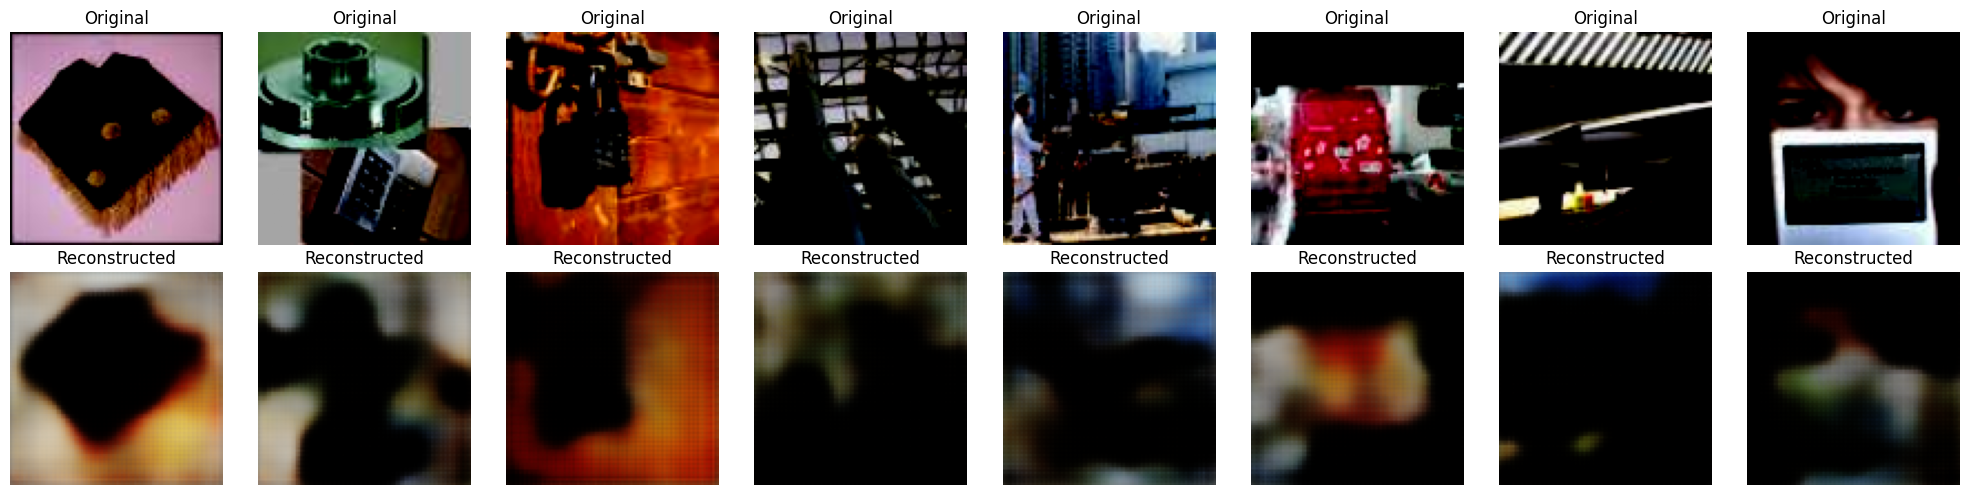
\includegraphics[width=\linewidth]{FIGURES/metatask/pn_rec.png} 
  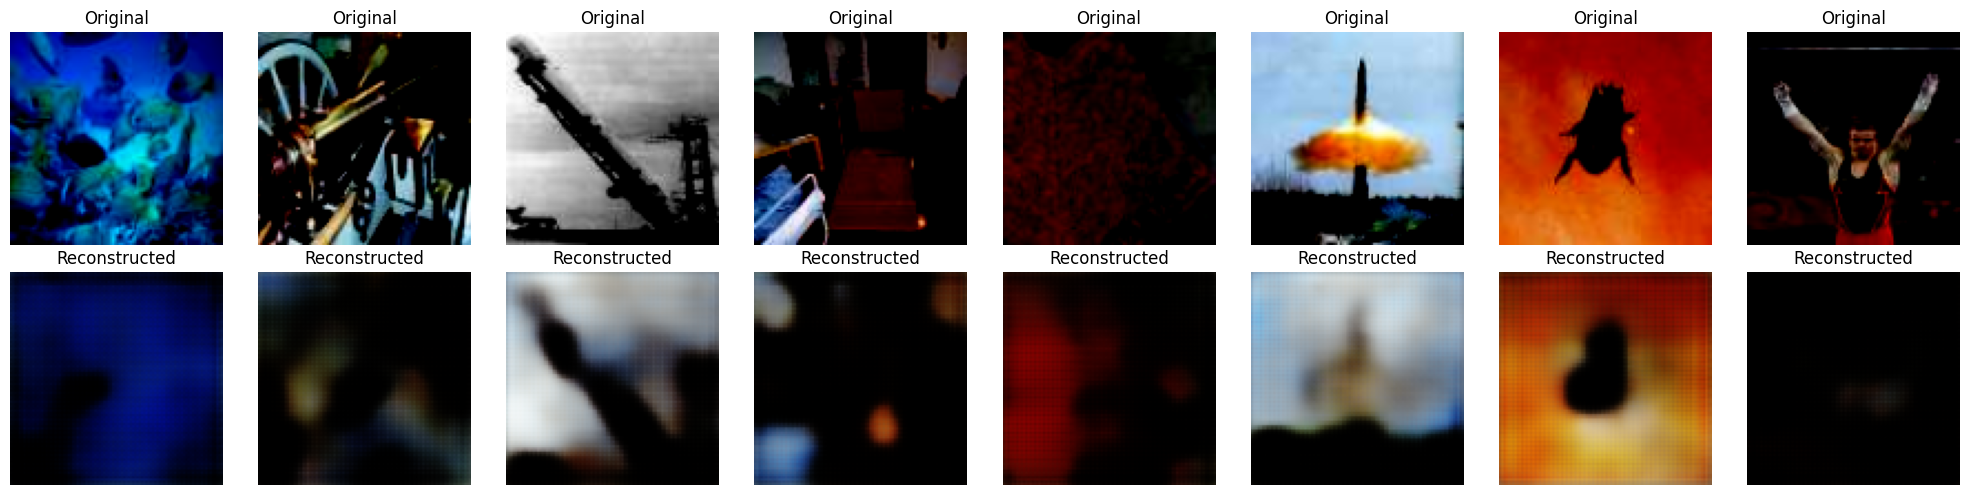
\includegraphics[width=\linewidth]{FIGURES/metatask/PN_rec_out_1.png}
  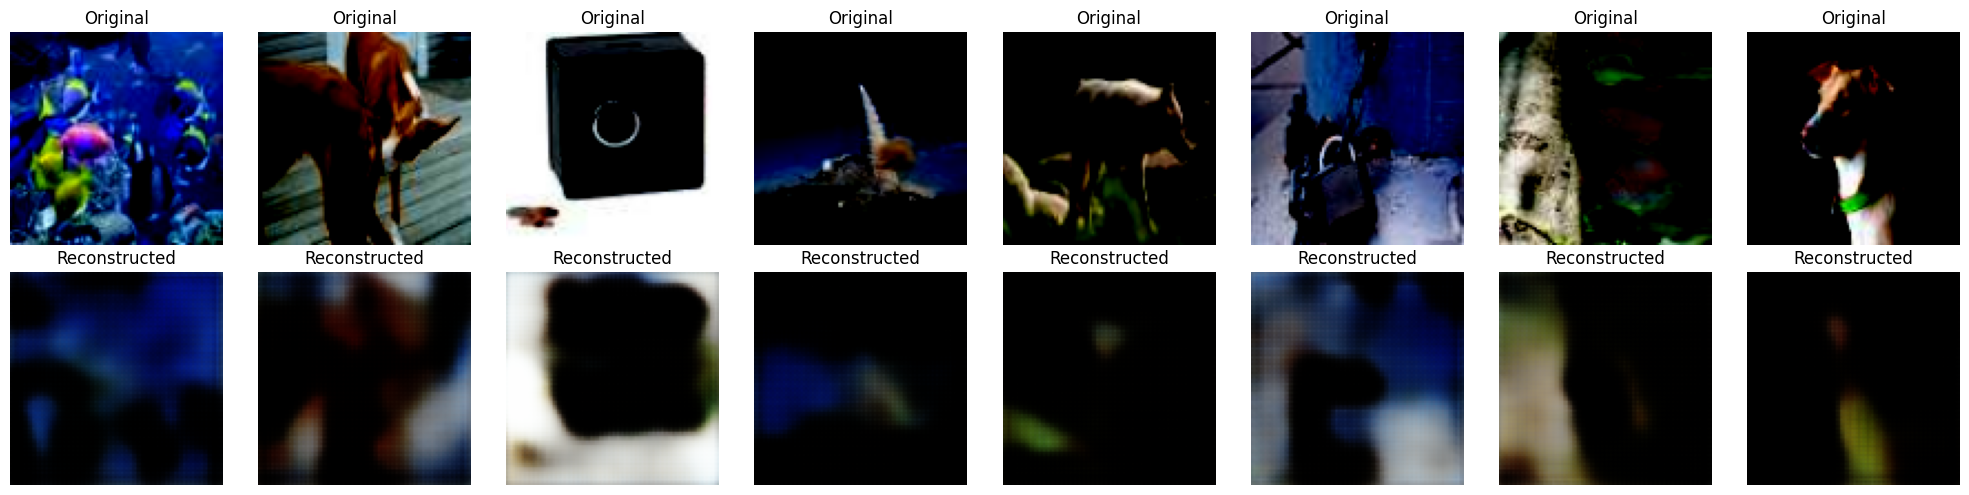
\includegraphics[width=\linewidth]{FIGURES/metatask/PN_rec_out_2.png}
  \caption{\color{black}The reconstruction results of the Prototypical Network integrated with the Task-Decoder, trained on TieredImageNet, are evaluated using MiniImageNet images.}
  \label{sup_fig:1}
\end{figure*}

\begin{figure*}[htbp]
  \centering
  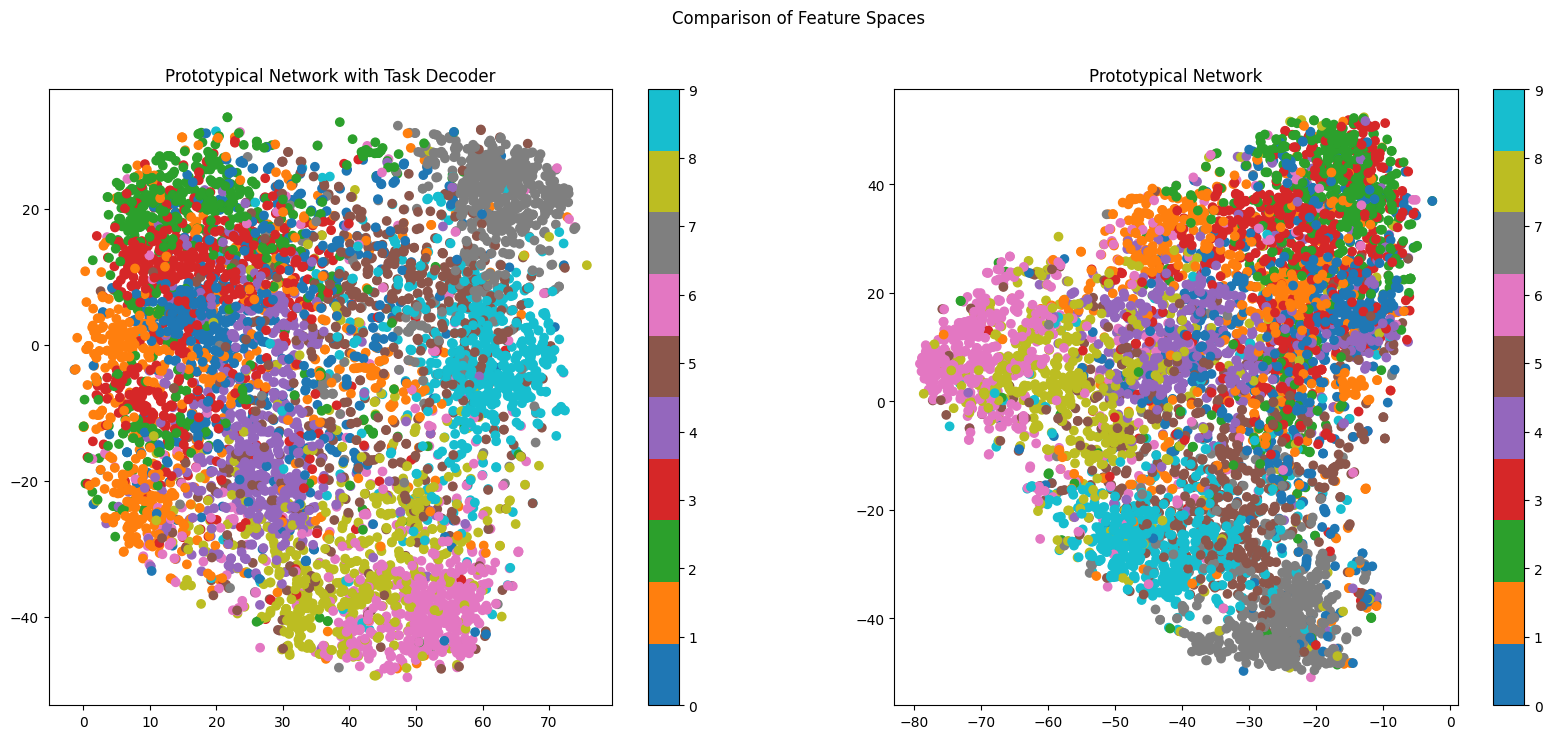
\includegraphics[width=\linewidth]{FIGURES/metatask/PNvsTD.png} 
  \caption{\color{black}illustrates the t-SNE projections of the first 10 classes of MiniImageNet for Prototypical Networks with (left) and without (right) the Task-Decoder. The integration of the Task-Decoder demonstrates enhanced class separability, indicating its effectiveness in improving feature representation.}
  \label{sup_fig:2}
\end{figure*}

\begin{figure*}[htbp]
  \centering
  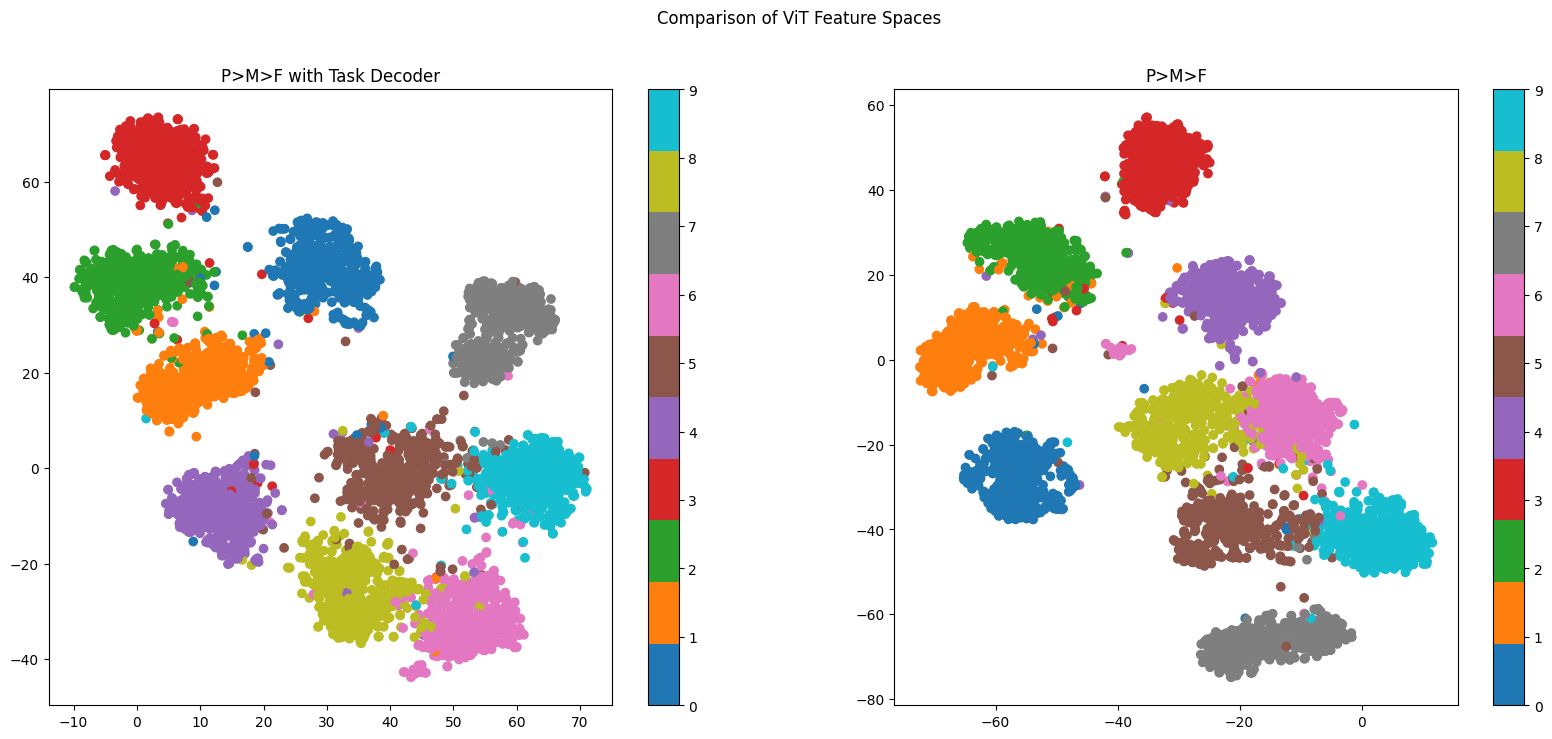
\includegraphics[width=\linewidth]{FIGURES/metatask/ViTPNvsTD.png} 
  \caption{\color{black}illustrates the t-SNE projections of the first 10 classes of MiniImageNet for P$>$M$>$F with (left) and without (right) the Task-Decoder. The integration of the Task-Decoder demonstrates enhanced class separability, indicating its effectiveness in improving feature representation.}
  \label{sup_fig:3}
\end{figure*}

\begin{figure*}[htbp]
  \centering
  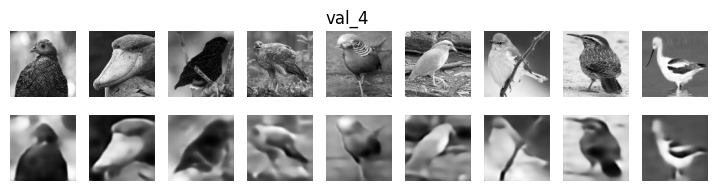
\includegraphics[width=0.8\linewidth]{FIGURES/metatask/autoencoder_val_4.png} 
  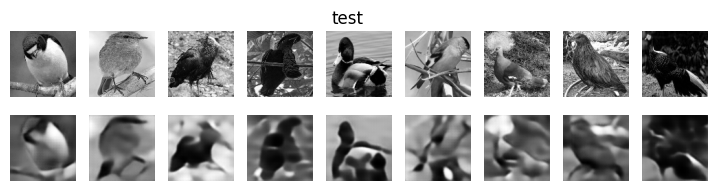
\includegraphics[width=0.8\linewidth]{FIGURES/metatask/autoencoder_test.png}
  \caption{\color{black}Reconstruction results ResNet Task Decoder before few-shot training.}
  \label{sup_fig:4}
\end{figure*}

\begin{figure*}[htbp]
  \centering
  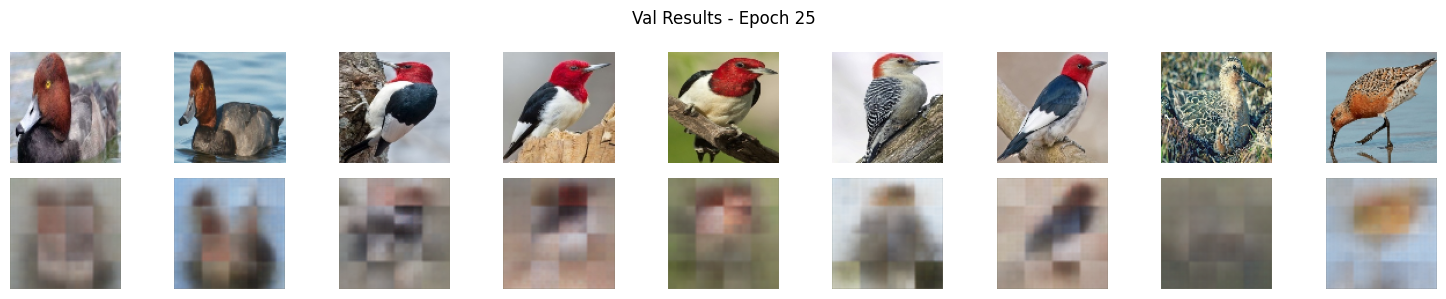
\includegraphics[width=\linewidth]{FIGURES/metatask/ViT_autoencoder_val.png} 
  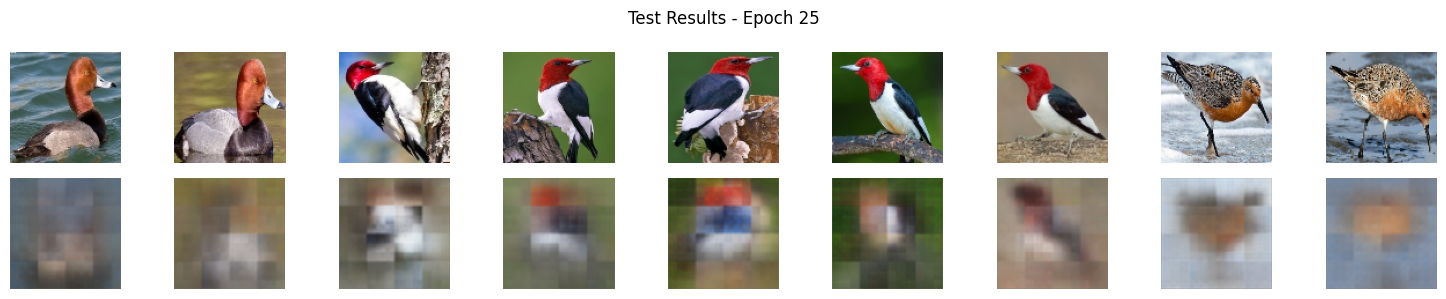
\includegraphics[width=\linewidth]{FIGURES/metatask/ViT_autoencoder_test.png}
  \caption{\color{black}Reconstruction results Task Decoder before few-shot training.}
  \label{sup_fig:5}
\end{figure*}

\begin{figure*}[htbp]
  \centering
  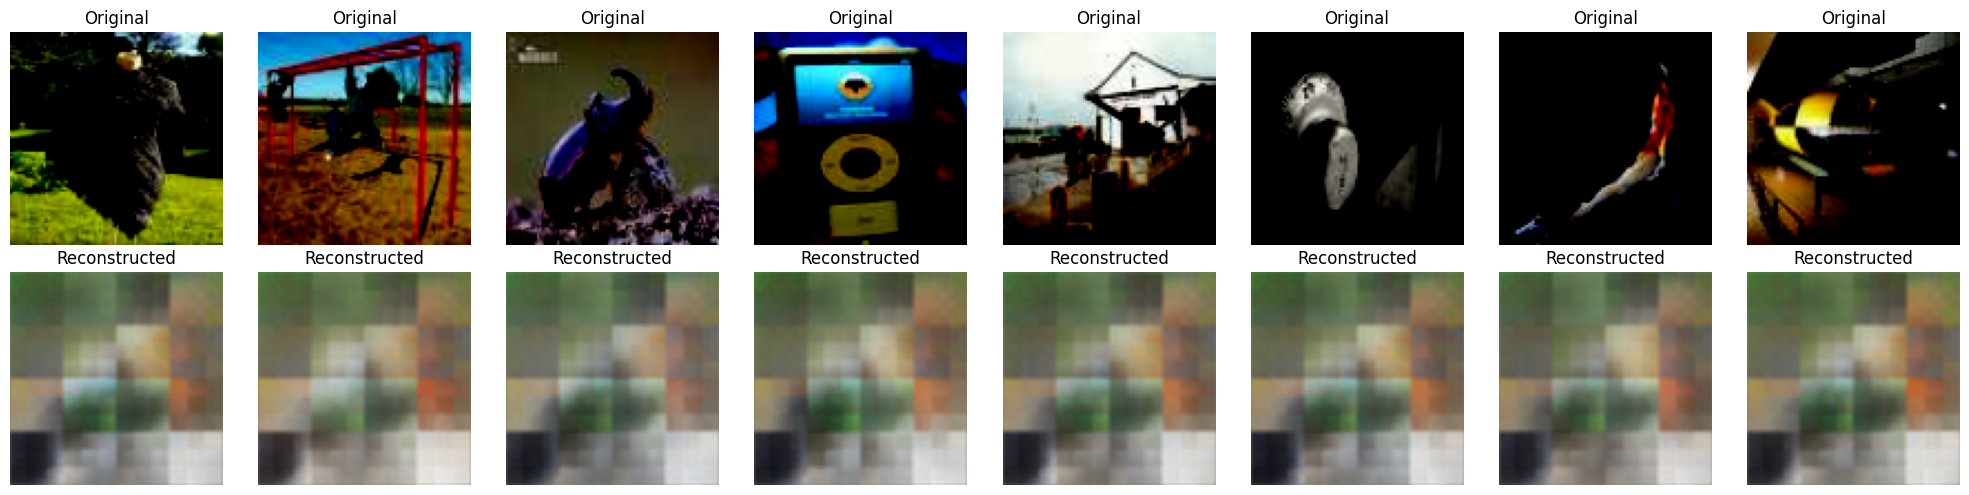
\includegraphics[width=\linewidth]{FIGURES/metatask/ViT_rec.png} 
  \caption{\color{black}Reconstruction results of P$>$M$>$F with ViT Task Decoder trained on MiniImageNet images.}
  \label{sup_fig:6}
\end{figure*}


\subsection{Extended Classification Results}
\label{sec:extended_results}

\subsubsection{Prototypical Networks}

We evaluated test accuracies using standard classification metrics and computed the F1-score to compare the performance of the two models. Tables~\ref{sup:2}, ~\ref{sup:3}, ~\ref{sup:8}, ~\ref{sup:9} present a comparison between Prototypical Networks and their Task-Decoder counterparts, demonstrating that the Task-Decoder exhibits significantly superior adaptation-generalization compared to Prototypical Networks. The F1-scores further indicate superior meta-generalization to novel tasks by the Task-Decoder.

\begin{table*}[htbp]
\centering
\caption{5-way 1-shot classification report of Precision (\%), Recall (\%), and F1-score (\%) on MiniImageNet using \textbf{Prototypical Networks} after 50,000 episodes.}
\label{sup:2}
\resizebox{\linewidth}{!}{%
\begin{tabular}{ccccc}
\hline
\textbf{Class} & \textbf{Support} & \textbf{Precision (\%)} & \textbf{Recall (\%)} & \textbf{F1-score (\%)} \\
\hline
0  & 46635  & 36.64 & 29.59 & 32.74 \\
1  & 44925  & 51.78 & 35.31 & 41.99 \\
2  & 37020  & 42.86 & 39.67 & 41.20 \\
3  & 30330  & 46.58 & 46.50 & 46.54 \\
4  & 44670  & 34.14 & 34.82 & 34.48 \\
5  & 29460  & 31.27 & 46.75 & 37.47 \\
6  & 36465  & 38.62 & 68.32 & 49.35 \\
7  & 44640  & 41.56 & 32.46 & 36.45 \\
8  & 22770  & 36.59 & 27.04 & 31.10 \\
9  & 14670  & 69.57 & 93.33 & 79.72 \\
10 & 36945  & 34.01 & 34.48 & 34.24 \\
11 & 38595  & 32.40 & 31.89 & 32.14 \\
12 & 37125  & 38.08 & 32.01 & 34.78 \\
13 & 59445  & 30.77 & 28.49 & 29.59 \\
14 & 46245  & 43.04 & 46.19 & 44.56 \\
15 & 44925  & 46.80 & 58.68 & 52.07 \\
17 & 67725  & 52.55 & 58.48 & 55.35 \\
18 & 29100  & 49.93 & 28.34 & 36.15 \\
19 & 38310  & 62.36 & 52.30 & 56.89 \\
\hline
\textbf{Accuracy (\%)}       & \multicolumn{4}{c}{42.90} \\
\textbf{Macro Average (\%)}  &        & 43.13 & 43.40 & 42.46 \\
\textbf{Weighted Average (\%)} &      & 42.45 & 42.20 & 41.64 \\
\hline
\end{tabular}%
}
\end{table*}

\begin{table*}[htbp]
\centering
\caption{5-way 1-shot classification report of Precision (\%), Recall (\%), and F1-score (\%) on MiniImageNet using \textbf{Prototypical Networks with Task-Decoder} after 50,000 episodes.}
\label{sup:3}
\resizebox{\linewidth}{!}{%
\begin{tabular}{ccccc}
\hline
\textbf{Class} & \textbf{Support} & \textbf{Precision (\%)} & \textbf{Recall (\%)} & \textbf{F1-score (\%)} \\
\hline
0  & 46635  & 40.08 & 31.99 & 35.58 \\
1  & 44925  & 57.97 & 47.64 & 52.30 \\
2  & 37020  & 53.45 & 43.70 & 48.09 \\
3  & 30330  & 59.32 & 52.89 & 55.92 \\
4  & 44670  & 40.26 & 37.58 & 38.87 \\
5  & 29460  & 45.57 & 58.67 & 51.30 \\
6  & 36465  & 45.14 & 73.41 & 55.90 \\
7  & 44640  & 45.68 & 41.21 & 43.33 \\
8  & 22770  & 53.30 & 36.17 & 43.09 \\
9  & 14670  & 66.96 & 96.80 & 79.16 \\
10 & 36945  & 39.39 & 38.42 & 38.90 \\
11 & 38595  & 41.17 & 39.37 & 40.25 \\
12 & 37125  & 44.74 & 39.99 & 42.23 \\
13 & 59445  & 36.32 & 36.61 & 36.46 \\
14 & 46245  & 45.68 & 46.86 & 46.26 \\
15 & 44925  & 53.66 & 54.31 & 53.98 \\
17 & 67725  & 53.84 & 67.44 & 59.88 \\
18 & 29100  & 45.04 & 31.58 & 37.13 \\
19 & 38310  & 56.64 & 56.94 & 56.79 \\
\hline
\textbf{Accuracy (\%)}       & \multicolumn{4}{c}{47.86} \\
\textbf{Macro Average (\%)}  &        & 48.64 & 49.03 & 48.18 \\
\textbf{Weighted Average (\%)} &      & 47.72 & 47.86 & 47.27 \\
\hline
\end{tabular}%
}
\end{table*}

\begin{table*}[htbp]
\centering
\caption{\color{black}5-way 5-shot classification report of Precision (\%), Recall (\%), and F1-score (\%) on MiniImageNet using \textbf{P$>$M$>$F with Task Decoder} after 3,000 episodes.}
\label{sup:8}
\resizebox{\linewidth}{!}{%
\begin{tabular}{c|c|c|c|c}
\hline
\color{black}\textbf{Class} & \color{black}\textbf{Support} & \color{black}\textbf{Precision (\%)} & \color{black}\textbf{Recall (\%)} & \color{black}\textbf{F1-score (\%)} \\
\hline
\color{black}0  & \color{black}2370  & \color{black}100.00 & \color{black}98.06 & \color{black}99.02 \\
\color{black}1  & \color{black}3420  & \color{black}95.95  & \color{black}93.45 & \color{black}94.68 \\
\color{black}2  & \color{black}4155  & \color{black}92.43  & \color{black}98.72 & \color{black}95.47 \\
\color{black}3  & \color{black}6270  & \color{black}96.52  & \color{black}88.60 & \color{black}92.39 \\
\color{black}4  & \color{black}3825  & \color{black}95.86  & \color{black}92.05 & \color{black}93.92 \\
\color{black}5  & \color{black}810   & \color{black}100.00 & \color{black}86.67 & \color{black}92.86 \\
\color{black}6  & \color{black}4320  & \color{black}88.03  & \color{black}98.87 & \color{black}93.13 \\
\color{black}7  & \color{black}795   & \color{black}100.00 & \color{black}100.00 &\color{black} 100.00 \\
\color{black}8  & \color{black}3135  & \color{black}96.94  & \color{black}94.93 & \color{black}95.92 \\
\color{black}9  & \color{black}5535  & \color{black}89.10  & \color{black}86.97 & \color{black}88.02 \\
\color{black}10 & \color{black}2970  & \color{black}90.49  & \color{black}94.78 & \color{black}92.58 \\
\color{black}11 & \color{black}3720  & \color{black}93.28  & \color{black}94.81 & \color{black}94.04 \\
\color{black}12 & \color{black}3810  & \color{black}92.72  & \color{black}90.31 & \color{black}91.50 \\
\color{black}13 & \color{black}4710  & \color{black}95.02  & \color{black}87.90 & \color{black}91.32 \\
\color{black}14 & \color{black}3330  & \color{black}88.83  & \color{black}87.15 & \color{black}87.98 \\
\color{black}15 & \color{black}5145  & \color{black}93.43  & \color{black}96.40 & \color{black}94.89 \\
\color{black}16 & \color{black}4080  & \color{black}89.26  & \color{black}90.44 & \color{black}89.85 \\
\color{black}17 & \color{black}5010  & \color{black}95.29  & \color{black}93.71 & \color{black}94.50 \\
\color{black}18 & \color{black}3600  & \color{black}87.67  & \color{black}81.58 & \color{black}84.52 \\
\color{black}19 & \color{black}3990  & \color{black}81.23  & \color{black}95.89 & \color{black}87.95 \\
\hline
\color{black}\textbf{Accuracy (\%)}       & \multicolumn{4}{c|}{\color{black}92.25} \\
\color{black}\textbf{Macro Average (\%)}  & \color{black}75000   & \color{black}93.10  & \color{black}92.57 & \color{black}92.73 \\
\color{black}\textbf{Weighted Average (\%)} & \color{black}75000 & \color{black}92.44  & \color{black}92.25 & \color{black}92.25 \\
\hline
\end{tabular}%
}
\end{table*}

\begin{table*}[htbp]
\centering
\caption{\color{black}5-way 5-shot classification report of Precision (\%), Recall (\%), and F1-score (\%) on MiniImageNet using \textbf{P$>$M$>$F} after 4,000 episodes.}
\label{sup:9}
\resizebox{\linewidth}{!}{%
\begin{tabular}{c|c|c|c|c}
\hline
\color{black}\textbf{Class} & \color{black}\textbf{Support} & \color{black}\textbf{Precision (\%)} & \color{black}\textbf{Recall (\%)} & \color{black}\textbf{F1-score (\%)} \\
\hline
\color{black}0  & \color{black}5700  & \color{black}98.35  & \color{black}96.18  & \color{black}97.25 \\
\color{black}1  & \color{black}5100  & \color{black}93.46  & \color{black}91.14  & \color{black}92.29 \\
\color{black}2  & \color{black}2460  & \color{black}97.81  & \color{black}96.18  & \color{black}96.99 \\
\color{black}3  & \color{black}2040  & \color{black}100.00 & \color{black}82.45  & \color{black}90.38 \\
\color{black}4  & \color{black}2685  & \color{black}95.23  & \color{black}89.16  & \color{black}92.09 \\
\color{black}5  & \color{black}4530  & \color{black}78.52  & \color{black}95.36  & \color{black}86.12 \\
\color{black}6  & \color{black}4965  & \color{black}95.35  & \color{black}95.91  & \color{black}95.63 \\
\color{black}7  & \color{black}1485  & \color{black}92.70  & \color{black}94.07  & \color{black}93.38 \\
\color{black}8  & \color{black}1635  & \color{black}100.00 & \color{black}63.55  & \color{black}77.71 \\
\color{black}9  & \color{black}3630  & \color{black}98.21  & \color{black}88.95  & \color{black}93.35 \\
\color{black}10 & \color{black}3105  & \color{black}92.10  & \color{black}93.88  & \color{black}92.98 \\
\color{black}11 & \color{black}2895  & \color{black}94.66  & \color{black}90.09  & \color{black}92.32 \\
\color{black}12 & \color{black}4785  & \color{black}92.77  & \color{black}92.54  & \color{black}92.66 \\
\color{black}13 & \color{black}4605  & \color{black}91.58  & \color{black}89.55  & \color{black}90.56 \\
\color{black}14 & \color{black}6090  & \color{black}85.71  & \color{black}89.36  & \color{black}87.50 \\
\color{black}15 & \color{black}2145  & \color{black}91.15  & \color{black}97.53  & \color{black}94.23 \\
\color{black}16 & \color{black}3900  & \color{black}88.29  & \color{black}94.74  & \color{black}91.40 \\
\color{black}17 & \color{black}4425  & \color{black}95.97  & \color{black}87.19  & \color{black}91.37 \\
\color{black}18 & \color{black}5040  & \color{black}80.83  & \color{black}79.48  & \color{black}80.15 \\
\color{black}19 & \color{black}3780  & \color{black}79.10  & \color{black}94.31  & \color{black}86.04 \\
\hline
\color{black}\textbf{Accuracy (\%)}       & \multicolumn{4}{c|}{\color{black}90.74} \\
\color{black}\textbf{Macro Average (\%)}  & \color{black}75000 & \color{black}92.09  & \color{black}90.08  & \color{black}90.72 \\
\color{black}\textbf{Weighted Average (\%)} & \color{black}75000 & \color{black}91.24  & \color{black}90.74  & \color{black}90.75 \\
\hline
\end{tabular}%
}
\end{table*}

\subsubsection{MAML}

Table~\ref{sup:4} provides a detailed comparison of the performance of MAML and Task-Decoder models on the MiniImageNet dataset. The table shows results for both 5-way 1-shot and 5-way 5-shot classification tasks across training, validation, and test sets. Notably, the Task-Decoder with a deeper CNN architecture consistently outperforms the standard MAML across all metrics, particularly in test accuracy, indicating its superior ability to generalize to unseen data. These results highlight the effectiveness of the Task-Decoder in improving model performance on few-shot learning tasks.

\begin{table*}[htbp]
\centering
\caption{Comparison of few-shot classification accuracies (\%) on MiniImageNet using MAML and Task-Decoder models. Results are reported for 5-way 1-shot and 5-way 5-shot settings, including Train, Validation, and Test accuracies.}
\label{sup:4}
\resizebox{\textwidth}{!}{%
\begin{tabular}{ll|ccc|ccc}
\hline
\multicolumn{2}{c|}{\textbf{Method}} & \multicolumn{3}{c|}{\textbf{5-way 1-shot (\%)}} & \multicolumn{3}{c}{\textbf{5-way 5-shot (\%)}} \\
\hline
\textbf{Model} & \textbf{Backbone} & \textbf{Train} & \textbf{Val} & \textbf{Test} & \textbf{Train} & \textbf{Val} & \textbf{Test} \\
\hline
MAML & CNN & 57.58 & 46.36 & 47.54 & 76.64 & 61.11 & 62.23 \\
\textbf{MAML (Task-Decoder)} & Shallow CNN & \textbf{58.10} & \textbf{45.24} & \textbf{47.81} & \textbf{76.82} & \textbf{61.04} & \textbf{62.52} \\
\textbf{MAML (Task-Decoder)} & CNN & \textbf{57.94} & \textbf{46.13} & \textbf{47.67} & \textbf{76.84} & \textbf{61.57} & \textbf{63.01} \\
\hline
\end{tabular}%
}
\end{table*}

\subsubsection{Computational Analysis}

To provide insights into the computational requirements of our approach, Table~\ref{sup:5} presents the training times for various model configurations. {\color{black}It is important to note that the reported times correspond to training for exactly 50,000 episodes. However, in practice, the Task-Decoder (TD) often converges in significantly fewer episodes, further highlighting its computational efficiency.}

\begin{table*}[htbp]
\centering
\caption{Comparison of training times (in hours) on MiniImageNet using MAML and Task-Decoder models for 5-way 1-shot and 5-way 5-shot experiments.}
\label{sup:5}
\resizebox{\textwidth}{!}{%
\begin{tabular}{ll|cc}
\hline
\textbf{Model} & \textbf{Backbone} & \textbf{5-way 1-shot} & \textbf{5-way 5-shot} \\
\hline
MAML & CNN & 5.1h & 7.2h \\
\textbf{MAML (Task-Decoder)} & Shallow CNN & \textbf{5.6h} & \textbf{7.9h} \\
\textbf{MAML (Task-Decoder)} & CNN & \textbf{6.4h} & \textbf{8.4h} \\
\hline
\end{tabular}%
}
\end{table*}

The Task-Decoder variants show consistently superior performance across metrics, particularly in test accuracy, while maintaining reasonable computational requirements. The deeper CNN architecture demonstrates the best overall performance, though at the cost of increased training time.

